\documentclass[11pt]{report}
\usepackage{geometry}
\geometry{
 a4paper,
 total={170mm,257mm},
 left=20mm,
 top=20mm,
 }
\usepackage[french]{babel}
\usepackage[T1]{fontenc}
\usepackage[utf8]{inputenc}
\usepackage{lmodern}
\usepackage{graphicx}
\usepackage{amssymb}
\usepackage{microtype}
\usepackage[colorlinks=true,
            linkcolor=red,
            urlcolor=blue,
            citecolor=blue]{hyperref}
            
\title{La simulation des fluides}
\author{Raoelisolonarivony - MISA M2}
\date{Décembre 2016}

\graphicspath{ {fluid-sims-images/} }

\begin{document}
\maketitle
\part{Les bases}

\section*{Description du cours}

L'animation des fluides comme l'eau, la fumée ou le feu par la simulation basée sur les lois de la physique croit en importance dans les effets visuels et commencent à avoir beaucoup d'impacts sur les jeux vidéos en temps réel. Ce cours part des bases des écoulement de fluide en 3D à son état-de-l'art dans la synthèse d'image. Nous commencerons par une explication intuitive des concepts importants sur la simulation de fluide, et suivant cette progression, démontrerons comment implémenter un système de simulation d'eau et de fumée effective, et compléterons les frontières en courbes irrégulières et  la tension de la surface. La dernière moitié du cours couvrira des sujets plus avancés comme les feux et explosions, la méthode des grilles adaptives, les algorithmes en temps réel couplés aux dernières technologies en accélération graphique, et les fluides dites non-newtonien comme le sable. 

\chapter{Les équations des fluides}
Les écoulement des fluides sont gouvernés par les fameuses équations des fluides incompressibles de Navier-Stokes. Cet ensemble d'équations aux dérivées partielles régit le comportement des fluides. Elles sont souvent écrites comme suit:

\begin{eqnarray}
\frac{\partial \overrightarrow{u}}{\partial t} + (\overrightarrow{u} . \nabla ) \overrightarrow{u} + \frac{1}{\rho} \nabla p & = & \overrightarrow{g} + \nu \nabla . \nabla \overrightarrow{u} \\
\nabla . \overrightarrow{u} & = & 0
\end{eqnarray}

\section{Les symboles}

Le symbole $ \overrightarrow{u} $ représente la vitesse du fluide. \newline

La lettre grecque $  \rho $ est la masse volumique du fluide. Pour l'eau, elle de l'ordre de $ 1000kg/m^3 $ tandis que pour l'air elle est de $ 1,3kg/m^3 $. \newline

La lettre \textit{p} pour "\textbf{pression}", représente la force exercée par le fluide sur une unité de surface. \newline

Le symbole \overrightarrow{g} est l'accélération de la pesanteur ayant comme coordonnées $(0; -9,81; 0) m/s^2 $ en prenant comme convention un axe $ y $ vertical et orienté vers le haut. \newline

La lettre grecque $\nu$ est appelé "\textbf{viscosité cinétique}". Elle mesure à quel point un fluide peut se déformer durant son écoulement. Par exemple le pois a une grande viscosité alors que l'alcool est un fluide à faible viscosité.

\section{L'équation d'inertie}

La première équation différentielle (1) est issue d'une équation vectorielle appelée "équation d'inertie". Cette équation est en fait celle de Newton $ \overrightarrow{F} = m. \overrightarrow{a} $ déguisée. Elle indique comment le fluide se meut soumis aux forces qui s'exercent sur lui. La seconde équation (2) est appelée "\textbf{condition d'incompressibilité}".

En supposant que l'animation d'un fluide est modélisée en utilisant un système de particules. Chaque particule représente alors un élément du fluide. Elle a une masse \textit{M}, un volume \textit{V} et une vitesse \overrightarrow{u}. Il faut dresser le bilan des forces appliquées sur la particule pour pouvoir obtenir la position de la particule après un temps donné. $ \overrightarrow{F} = m. \overrightarrow{a} $ donne ensuite l'accélération pour créer le mouvement de cette particule. Cette accélération s'écrit:

\begin{eqnarray}
\overrightarrow{a} & = & \frac{D \overrightarrow{u}}{Dt}
\end{eqnarray}

La loi de Newton devient:

\begin{eqnarray}
\overrightarrow{F} & = & m. \frac{D \overrightarrow{u}}{Dt}
\end{eqnarray}

Quant aux forces s'exerçant sur la particule, la plus évidente est la force de la gravité $ m\overrightarrow{g} $. Les autres particules du fluide exerçent aussi des forces sur la particule concerné. \newline

La première est la pression. Les régions à haute pression refoulent celles à basse pression. Ce qui est intéressant est la somme des forces appliquées à la particule. Par exemple, si la particule est soumise à une pression égale dans toutes les directions, la somme des forces sera nulle. Ce qui compte surtout c'est l'influence d'une haute pression sur un côté particulier de la particule, entrainant une force dirigée depuis les zones à haute pression vers celles à basse pression. La plus simple manière de mesurer la différence de pression sur la particule à une position donnée est de calculer la valeur du gradient de pression avec le signe moins: $ - \nabla p $.
L'intégrale de cet élément sur le volume entier du fluide donne la force de pression. Par approximation, il est possible de multiplier par le volume V. En fait, la pression garde le volume du fluide constant.\newline

L'autre force exercée par le fluide sur une de ses particules est celle due à la viscosité. Un fluide visqueux tend à résister à la déformation. C'est une force qui pousse la particule avec une vitesse, qui est la moyenne des vitesses des particules voisines, c'est-à-dire qu'elle cherche à minimiser les différences de vitesses entre les particules voisines dans le fluide. L'opérateur différentiel qui mesure à quelle proportion une quantité varie autour de la moyenne est le laplacien $ \nabla . \nabla $. L'intégration de cette valeur sur le volume entier donne la force due à la viscosité. Le "\textbf{coefficient de viscosité dynamique}" est noté $ \mu $. Ce coefficient est en rapport à la force plutôt qu'à l'accélération.\newline

En regroupant toutes les forces et en remplaçant dans l'équation (4), le mouvement de la particule est régit par l'équation suivante:

\begin{eqnarray}
m\overrightarrow{g} - V \nabla p + V \mu \nabla . \nabla \overrightarrow{u} & = & m. \frac{D \overrightarrow{u}}{Dt}
\end{eqnarray}

Evidemment, le fait d'approximer le fluide en ne prennant compte qu'un nombre fini d'éléments est sujet à erreur. La limite à fixer se fait au niveau de la taille des particules qui doit tendre vers zero et le nombre de particules dans le fluide qui doit tendre vers l'infini. L'équation du mouvement de la particule est affecté par ces limitations puisque la masse \textit{m} et le volume \textit{V} vont tendre vers zéro.
En divisant membre à membre l'équation (5) par le volume, la masse volumique entre en jeu et règle le problème des limites. Cette équation, en tenant compte que la masse volumique $ \rho $ = $ \frac{m}{V} $, devient:

\begin{eqnarray}
\rho\overrightarrow{g} - \nabla p + \mu \nabla . \nabla \overrightarrow{u} & = & \rho. \frac{D \overrightarrow{u}}{Dt}
\end{eqnarray}

En divisant ensuite par la masse volumique $ \rho $, cela donne:

\begin{eqnarray}
\overrightarrow{g} - \frac{1}{\rho}\nabla p + \frac{\mu}{\rho} \nabla . \nabla \overrightarrow{u} & = & \frac{D \overrightarrow{u}}{Dt}
\end{eqnarray}

En définissant la viscosité cinématique par $ \nu = \frac{\mu}{\rho} $, l'équation devient:

\begin{eqnarray}
\overrightarrow{g} - \frac{1}{\rho}\nabla p + \nu \nabla . \nabla \overrightarrow{u} & = & \frac{D \overrightarrow{u}}{Dt}
\end{eqnarray}

L'équation d'inertie (1) est sensiblement retrouvée. En fait, l'utilisation de la dérivée totale $ \frac{D\overrightarrow{u}}{Dt} $ est plus importante pour la synthèse d'image et nous conduit à des méthodes de résolutions numériques de l'équation. Pour expliciter cette importance de la dérivée $ \frac{D\overrightarrow{u}}{Dt} $, il faut considérer les approches de résolution "\textbf{Lagrangien} " et "\textbf{Eulérien}". 

\section{Les points de vue Lagrangienne et Eulérienne}

Le mouvement des fluides et des solides déformables peut être décrit en suivant deux approches: Lagrangienne et Eulérienne.\newline

L'approche Lagrangienne (en l'honneur du mathématicien français Joseph Louis Lagrange) gère ce mouvement comme un système de particules. Chaque point dans le fluide est étiquetté comme une particule séparée, avec sa position \overrightarrow{x} et sa vitesse \overrightarrow{u}. On peut raisonnablement considérer la particule comme une molécule du fluide. Les fluides sont simulés par l'approche de Lagrange en un ensemble discret de particules connectées par des mailles, comme le sont communément les solides déformables.\newline

L'approche Eulérienne (en l'honneur du mathématicien suisse Leonhard Euler), suit une tactique différente. Il est habituellement lié à la description du mouvement des fluides. Au lieu de retracer chaque particule, on s'intéresse à des points fixes dans l'espace et on note l'évolution des caractéristiques du fluide (comme la masse volumique, la vitesse, la température, etc.) au cours du temps en ces points. Quand le fluide s'écoule à travers ces points, il contribue au changement de ces caractéristiques (par exemple, quand un fluide chaud qui refroidit traverse les points, la température diminue - même si la température de chaque particule du fluide reste constante). \newline

Une façon de comprendre les deux approches est son assimilation à la collecte de données météorologique. Pour la méthode de Lagrange, le point de vue se situe et se déplace dans un ballon laissé flotté au gré du vent et mesurant au passage la pression, la température et l'humidité de l'air aux alentours. Pour la méthode d'Euler, le point de vue est fixé sur le sol, mesurant la pression, la température et l'humidité de l'air qui transite par le point de vue. \newline

D'un point de vue numérique, la méthode de Lagrange correspond à un système de particules (avec ou sans maillage) et la méthode d'Euler consiste à utiliser une grille fixe dans l'espace qui ne change pas même si le fluide le traverse. \newline

L'approche eulérienne, malgré son apparente difficulté, est privilégié par rapport à celle de Lagrange pour les raisons suivantes:

\begin{enumerate}
\item Gérer les dérivées comme le gradient de la pression ou la viscosité est analytiquement aisé; 
\item L'approximation de ces dérivées dans un système eulérien est plus pratique que dans un nuage de particules suivant des mouvements arbitraires.\newline
\end{enumerate}

La connexion liant les deux points de vue est la dérivée totale $ \frac{Dq}{Dt} $. D'abord pour le point de vue de Lagrange, le fluide est composé de particules avec des positions \overrightarrow{x} et des vitesses \overrightarrow{u}. En supposant que le fluide possède un caractère \textit{q}, chaque particule possède une valeur pour \textit{q} ( \textit{q} peut être la masse volumique, la vitesse, la température ou tout autre caractéristique du fluide). En particulier, la function $ q(t,\overrightarrow{x}) $ indiquant la valeur de \textit{q} à un instant \textit{t} pour la particule situé à une position $ \overrightarrow{x} $ représente une variable d'Euler. La variation de la caractéristique \textit{q}  de la particule répond quant à elle à la question de Lagrange. En prenant la dérivée totale:

\begin{eqnarray}
\frac{d}{dt} q(t, \overrightarrow{x}) 
& = & \frac{\partial q}{\partial t} + \nabla q. \frac{d\overrightarrow{x}}{dt} \\
& = & \frac{\partial q}{\partial t} + \nabla q. \overrightarrow{u} \\
& = & \frac{Dq}{Dt}
\end{eqnarray}

Les deux termes intervenants dans cette dérivée sont $ \frac{\partial q}{\partial t} $ et  $ \nabla q. \overrightarrow{u} $ dans l'égalité (10). Le premier terme indique à quelle vitesse \textit{q} varie dans une position fixé dans l'espace (une mesure eulérienne). Le second terme corrige la variation occasionée à cette position qui n'a été causé que par les différences des fluides ayant transités par cette position (exemple: le changement de température vient du fait que le fluide froid s'est substitué au fluide chaud, il n'est pas causé par un changement de température des molécules).

Finallement, en 3D et en fonction de ses dérivées partielles, cette dérivée s'écrit:

\begin{equation}
\frac{Dq}{Dt} 
 =  \frac{\partial q}{\partial t} + u \frac{\partial q}{\partial x} + v \frac{\partial q}{\partial y} + w \frac{\partial q}{\partial z}
\end{equation}
 
La discussion porte sur la manière dont la particule fluide, ayant un caractère \textit{q}, est en mouvement dans un champ de vecteur vitesse \overrightarrow{u}. C'est ce qu'on appelle communément "\textbf{advection}" (ou parfois "\textbf{convection}" ou "\textbf{transport}"). Une "\textbf{équation d'advection}" utilise la dérivée $ \frac{Dq}{Dt} $, telle quelle soit nulle:

\begin{eqnarray}
\frac{Dq}{Dt} & = & 0 \\
\frac{\partial q}{\partial t} + \nabla q. \overrightarrow{u} & = & 0
\end{eqnarray}

Cela signifie juste que la caractéristique q varie, mais pas au sens du point de vue de Lagrange.

\subsection{Exemple}

Pour simplifier, un exemple en une dimension est préférable sans fausser les raisonnements. Soit la caractéristique \textit{T} représentant la température du fluide. En supposant qu'à un instant \textit{t}, la température soit donnée par: 

\begin{eqnarray*}
T(x) = 10 x
\end{eqnarray*}

La température est de 0 (en degré Celsius) à l'origine et augmente au fur et à mesure que l'on avance vers la droite du repère, jusqu'à une température limite de 100 pour $x = 10 $. En supposant qu'un vent souffle à une vitesse \textit{c},  en d'autre termes que partout la vitesse du fluide est \textit{c}:

\begin{eqnarray*}
\overrightarrow{u} = c
\end{eqnarray*}

La température de chaque particule d'air est supposée constante, les particules sont seulement en mouvement. Donc, suivant l'approche de Lagrange, la variation de température est nulle:

\begin{eqnarray*}
\frac{DT}{Dt} = 0
\end{eqnarray*} 

En développant, cette équation devient:

\begin{eqnarray*}
\frac{\partial T}{\partial t} + \nabla T.\overrightarrow{u} & = & 0 \\
\frac{\partial T}{\partial t} + 10.c & = & 0 \\
\frac{\partial T}{\partial t}  & = & - 10.c
\end{eqnarray*} 

Interprétation: Pour un point fixé dans l'espace, la température varie avec le taux $ -10c $. Si le vent s'arrête de souffler, $ c = 0 $, rien ne change. Si le vent souffle vers la droite avec une vitesse $ c = 1 $, la température descendra à $ -10 $. Si par contre le vent souffle vers la gauche avec une vitesse $ c = -2 $, la température à ce point augmentera à 20. Dans ce cas, même si la dérivée de Lagrange est nulle, celle d'Euler peut prendre différentes valeurs dépendant de la vitesse et de la direction du fluide en mouvement. 


\subsection{Quantité de vecteur d'advection}

Une confusion apparaît pour l'application de l'opérateur de dérivée $ \frac{D}{Dt} $ sur la caractéristique de type vecteur, la coulour RGB par exemple, et encore plus de confusion pour son application sur le vecteur vitesse \overrightarrow{u}. Pour l'éviter, il faut prendre chaque composante séparemment.

Pour le vecteur de couleur $ \overrightarrow{C} = (R, G, B) $, la dérivée s'écrit:
\[
\frac{D\overrightarrow{C}}{Dt} = 
  \left[
	\begin{array}{c}
		DR/Dt\\
		DG/Dt\\
		DB/Dt
	\end{array}
 \right] = 
 \left[
	\begin{array}{c}
		\partial R/\partial t + \overrightarrow{u} . \nabla R \\
		\partial G/\partial t + \overrightarrow{u} . \nabla G \\
		\partial B/\partial t + \overrightarrow{u} . \nabla B
	\end{array}
 \right] = 
 \frac{\partial \overrightarrow{C}}{\partial t} + \overrightarrow{u} . \nabla \overrightarrow{C}
\]

Le terme $ \overrightarrow{u} . \nabla \overrightarrow{C} $ est un abus de notation, il représente implicitement l'advection du vecteur couleur $\overrightarrow{C} $ suivant ses composantes scalaires.

De même, l'advection de la vitesse $ \overrightarrow{u} = (u, v, w) $ s'écrit:

\[
\frac{D\overrightarrow{u}}{Dt} = 
  \left[
	\begin{array}{c}
		Du/Dt\\
		Dv/Dt\\
		Dw/Dt
	\end{array}
 \right] = 
 \left[
	\begin{array}{c}
		\partial u/\partial t + \overrightarrow{u} . \nabla R \\
		\partial v/\partial t + \overrightarrow{u} . \nabla G \\
		\partial w/\partial t + \overrightarrow{u} . \nabla B
	\end{array}
 \right] = 
 \frac{\partial \overrightarrow{u}}{\partial t} + \overrightarrow{u} . \nabla \overrightarrow{u}
\]

En développant, cette formule s'écrit:
\[
\frac{D\overrightarrow{u}}{Dt} = 
  \left[
	\begin{array}{c}
		\partial u/\partial t + u \partial u / \partial x + v \partial u / \partial y + w \partial u / \partial z \\
		\partial v/\partial t + u \partial v / \partial x + v \partial v / \partial y + w \partial v / \partial z\\
		\partial w/\partial t + u \partial w / \partial x + v \partial w / \partial y + w \partial w / \partial z
	\end{array}
 \right]
\]

\section{L'incompressibilité}

Les fluides réels, même l'eau, peut changer de volume. En fait, les ondes de son résultent de perturbation du volume (de la masse volumique et la pression) du fluide. Une fausse affirmation stipule que la différence entre les liquides et les gaz est que les gaz pouvaient changer de volume et pas les liquides. Cette affirmation peut être réfuté par le fait qu'il possible d'entendre sous l'eau.

Un point crucial cependant, les fluides ne changent de volume qu'à très petit échelle. Il est presque impossible de modifier le volume de l'eau même avec une puissante pompe à eau. L'air même ne change pas de volume sauf s'il est fixé à une pompe ou dans d'extrêmes situations comme quand un objet franchit le mur du son. L'étude se rapportant à l'étude de tels phénomènes est celle des "\textbf{fluides compressibles}". L'écoulement de tels fluides est compliqué et couteux à simuler, et hormis pour l'acoustique, n'entre pas en jeu dans la vie quotidienne. De même, les ondes de son ne représentent qu'une infime partie des perturbations de volume, et ont des effets négligeables sur le mouvement des fluides à un niveau macroscopique (eau débarbouillante, fumée tournoyante, etc.), et n'ont donc pas une importance sur l'animation.

Pour l'animation, les fluides sont considérés "\textbf{imcompressibles}", c'est-à-dire que leur volume ne change pas.
Mathématiquement, en prenant une volume de fluide $ \Omega $ quelconque à un instant donné, de frontière $ \partial\Omega $, la mesure de la progression du volume de fluide est obtenue en intégrant la composante normale de sa vitesse suivant cette frontière:

\begin{equation}
\frac{d}{dt} Volume(\Omega) = \int \!\!\!\! \int_{\partial \Omega} \overrightarrow{u} . \hat{n}
\end{equation}

Pour un fluide incompressible, le volume est constant, l'équation (15) devient:

\begin{equation}
\int \!\!\!\! \int_{\partial \Omega} \overrightarrow{u} . \hat{n} = 0
\end{equation}

En utilisant le théorème de la divergence, l'équation fait apparaitre l'intégrale sur le volume:

\begin{equation}
\int \!\!\!\! \int \!\!\!\! \int_{\Omega} \nabla . \overrightarrow{u} = 0
\end{equation}

Toute la magie vient du fait que cette équation doit être toujours vraie quelque soit le volume $ \Omega $ pris dans l'ensemble du fluide. La seule fonction qui s'annule en s'intégrant indépendamment du volume choisi est la fonction nulle. En conséquence, l'équation (17) se réduit comme suit:

\begin{eqnarray*}
\mathbf{\nabla . \overrightarrow{u} = 0}
\end{eqnarray*}

L'équation (2) est retrouvée, elle s'appelle "\textbf{Equation d'incompressibilité}" du fluide. c'est la deuxième partie des équations de Navier-Stokes.
Le champ de vecteur qui vérifie cette équation d'incompressibilité est appelé "\textbf{champ incompressible}" ou "\textbf{champ solénoïdal}" ou "\textbf{champ à divergence zéro}". Une des parties les plus sensibles lors de la simulation de fluide est de préserver cette incompressibilité pour le champ de vecteur de vitesses. C'est là que la pression entre en jeu.

Une façon de considérer la pression est que c'est la force qui permet de préserver l'incompressibilité de la vitesse.

La pression intervient uniquement dans l'équation d'inertie (1), il faut trouver une relation qui lie la pression avec la divergence du champ de vitesse. En appliquant la divergence aux deux membres de l'équation d'inertie, on a l'équation suivante:

\begin{equation}
\nabla . \, \frac{\partial \overrightarrow{u}}{\partial t} + \nabla . \, (\nabla \overrightarrow{u}. \,  \overrightarrow{u}) + \nabla . \, \frac{1}{\rho} \nabla p  =  \nabla . \, (\overrightarrow{g} + \nu \nabla . \nabla \overrightarrow{u})
\end{equation}

En inversant les opérateurs de dérivation dans le premier terme de cette équation, c'est-à-dire:

\begin{equation}
\frac{\partial }{\partial t}\nabla .\overrightarrow{u}
\end{equation}

Et en considérant que terme doit être nul compte tenu de la contrainte d'incompressibilité, le réarrangement de l'équation (18) donne:

\begin{equation}
\nabla . \frac{1}{\rho}\nabla p = \nabla . (-\nabla \overrightarrow{u} . \overrightarrow{u}+ \overrightarrow{g} + \nu \nabla . \nabla \overrightarrow{u}) 
\end{equation}


\section{Négliger la viscosité}	

Dans certaines situations, la viscosité tient un rôle important: pour la simulation de miel ou de gouttes d'eau par exemple. Seulement, pour la plupart des animations, la viscosité joue un rôle de moindre importance. Sa simplification dans l'équation bénificie l'équation de Navier-Stokes de practicité. En fait, la plupart des méthodes numériques intervenants dans la simulation de fluides prônent des erreurs interprétables comme étant due à la viscosité du fluide. Donc le fait d'enlever le terme de viscosité dans l'équation ne nuit pas à la simulation. 

Les équations de Navier-Stokes privées des termes portant sur la viscosité sont appelées "\textbf{Equation d'Euler}", et un fluide dit parfait sans viscosité est qualifié de fluide "\textbf{invisqueux}". Les équations résultant de la suppression des termes mettant en jeu la viscosité sont les suivantes:

\begin{eqnarray}
\frac{D\overrightarrow{u}}{Dt} + \frac{1}{\rho} \nabla p & = & \overrightarrow{g} \\
\nabla . \overrightarrow{u} & = & 0
\end{eqnarray}

Ce sont les équations les plus utilisées dans l'animation.

\section{Conditions à la frontière}	

Une des choses les plus intéressantes dans la simulation numérique des fluides est la description du mouvement du fluide aux frontières. 

Deux frontières usuellement rencontrées sont les frontières dites "parois solides" et "surfaces libres". Les frontières impliquant la frontière entre deux fluides différents sont aussi importantes: il est rare d'en avoir besoin en animation. Un article travaillant sur ces frontières où deux fluides entrent en collision est celui de Jeong-Mo Hong and Chang-Hun Kim \cite{Hong-05}.

Une frontière en paroi solide est là où le fluide entre en contact avec un solide. En terme de vitesse: A la frontière, le fluide ne doit pas pénétrer à travers le solide ou en sortir s'il y est contenu, donc la composante normale de la vitesse à cet emplacement est nulle:

\begin{equation}
\overrightarrow{u}.\hat{n} = 0
\end{equation}

L'équation (23) s'applique surtout si le solide n'est pas en mouvement. Dans le cas général, la composante normale de la vitesse du fluide doit correspondre à la composante normale de la vitesse du solide à son contact, c'est-à-dire:

\begin{equation}
\overrightarrow{u}.\hat{n} = \overrightarrow{u}\!\!_{solid} \,.\, \hat{n}
\end{equation}

Dans les deux équations, $ \hat{n} $ est la normale à la frontière solide.
Ces équations représentent les conditions qui évitent au fluide de coller au solide, étant donné que la composante normale de la vitesse est restreinte, ce qui permet au fluide de glisser en suivant la direction tangentielle.\newline

Quant est-il de la pression sur la frontière entre le fluide et le solide? L'idée de départ est que c'est la pression qui "maintient le fluide dans son état incompressible" en préservant son volume. Il faut aussi que les conditions aux frontières de type "parois solides" soient respectées. Le terme $ \frac{1}{\rho}\nabla p$ de l'équation d'inertie s'applique aussi à la frontière. Ainsi, la pression peut contrôler $  \overrightarrow{u} \,.\, \hat{n} $ au paroi solide, ce qui indique une propriété de $ \nabla p \,.\, \hat{n} $, aussi appelée la dérivée normale de la pression "$ \partial p / \partial \hat{n} $".\newline

Que se passerait-il si le liquide était visqueux? Les frottements dus à la viscosité auront une influence sur la composante tangentielle de la vitesse du fluide. Le cas le plus simple est la condition de non-glissement de la frontière, spécifiant:

\begin{equation}
\overrightarrow{u} = 0
\end{equation}

et si le solide est en mouvement, la condition est:

\begin{equation}
\overrightarrow{u} \,=\, \overrightarrow{u}\!\!_{solid}
\end{equation}

Parfois, la frontière en parois solides est un genre d'évent ou un drain que le fluide peut traverser. Dans ce cas, le produit $ \overrightarrow{u}\,.\,\hat{n} $ doit être différent de la vitesse de la frontière, il doit plutôt être égale à la vitesse d'aspiration ou de refoulement du conduit dans la simulation.\newline


Le deuxième type de frontière est celle entre le fluide et la surface libre ou surface ouverte. C'est l'ensemble des points où la modélisation du fluide n'est pas prise en compte. Par exemple, dans le cas de la simulation de l'eau qui éclabousse, les surface de l'eau qui \textbf{ne sont pas} en contact avec le solide sont les surfaces libres. En réalité, l'eau est en contact avec un autre fluide qui est l'air, mais cela ajoute plus de complexité  pour ajouter la simulation de l'air dans l'équation. De plus, comme l'air est 700 fois plus léger que l'eau, il n'a pas un effet assez significatif sur l'eau. Donc, l'air est modélisé simplement comme étant une région avec une pression atmosphérique. Et puisque pour les fluides incompressibles, seules les \textbf{ différences} de pression comptent, la pression constante de l'air peut être choisi arbitrairement: zéro fait bien l'affaire. En conséquence, une surface ouverte est celle qui a une pression $ p = 0 $, et la vitesse y est hors de contrôle.\newline

Un autre cas où la surface ouverte est importante est celui de la simulation d'une petite partie de fluide qui fait partie d'un domaine plus large: par exemple la simulation de la fumée dans l'air. Simuler l'atmosphère tout entier n'est pas envisageable, donc une limitation sur une grille qui engloge la "zone d'intérêt" est fixée pour la simulation. A la frontière de cette zone, le fluide doit continuer, mais la simulation ne dépasse pas cette limite. Seulement, comme la simulation laisse le fluide pénétrer ou sortir de cette zone, la frontière est considérée comme une surface ouverte, $ p = 0 $, même si il n'y a aucune surface visible.\newline

Un dernier point sur les surfaces libres: pour les liquides de petites grandeurs, la tension surfacique peut être importante. Dans les couches intérieures moléculaires, la tension de surface existe à cause de la variation des forces d'attraction entre les molécules de différents types. Par exemple, les molécules d'eau sont fortement attirés  plus par les autres molécules d'eau que par les molécules d'air: en conséquence, les molécules d'eau sur la surface séparant l'air et l'eau tendent à être entourés par encore plus d'eau autant que possible que d'air. Sur le point de vue géométrique, les chimistes ont modélisé ce phénomène par l'action de forces cherchant à minimiser la surface, ou à réduire la courbure moyenne de la surface. En d'autres mots, c'est la tension qui essaye constamment à rétrécir la surface, d'où son nom de tension de surface. L'autre manière d'interpréter cette tension est basée sur la courbure moyenne de la surface.\newline

Pour faire court, le modèle à considérer est celui qui prend en compte qu'il y a un saut de pression entre les deux fluides en contact, qui est proportionnel à la courbure moyenne:

\begin{equation}
[p] = \gamma \kappa
\end{equation}

La notation $ [p] $ représente le saut de pression en question, c'est-à-dire la différence de pression mesurée sur le côté de l'eau et celle mesurée sur le côté de l'air, $ \gamma $ est le coefficient de la tension de surface ( pour l'air et l'eau à la température à l'ombre, il est approximativement $ \gamma \approx 0.073 N/m $), et $ \kappa $ est la courbure moyenne, mesurée en $ 1/m $. Ce qui signifie que pour une surface ouverte avec une tension de surface, la pression à la surface de l'eau est la somme  de la pression de l'air ($0 Pa$) et du saut de pression:

\begin{equation}
p = \gamma \kappa
\end{equation}

Les surfaces libres présentent un problème majeur: les bulles d'air se rompent immédiatement. Même si l'air est plus léger que l'eau, et qu'il ne peut pas transférer beaucoup d'élan à l'eau, il demeure incompressible. Une bulle d'air dans l'eau garde son volume. Modéliser une bulle d'air comme une surface ouverte provoquerait l'explosion de l'air. Pour pallier ce problème, une possibilité est de simuler en ajoutant des bulles d'air à la surface ouverte, ou plus généralement simuler l'air et l'eau (simulation à deux phases étant donné les deux fluides).

\chapter{Revue des simulations numériques}

Ayant ces équations de bases sur la mécanique des fluides, comment les discretiser ses équations numériquement pour la simulation sur ordinateur? Il y a plusieurs options pour cette numérisation, et encore aujourd'hui des innovations sur le sujet continuent de se multiplier.

\section{La décomposition}

Il s'agit de décomposer une équation complexes en parties plus petites résolues séparémment. Par exemple, si le caractéristique est la somme de différentes termes, l'opération consister à calcul chaque terme en premier temps, et à faire la somme des résultats donne la solution.

Pour plus d'éclaircissement, prenons l'exemple très simple d'une équation différentielle du premier degré:

\begin{eqnarray}
\frac{dq}{dt} = 1 + 2
\end{eqnarray}

La solution est évidemment $ q(t) = 3t + q(0) $. Mais, par décomposition, deux étapes principales sont nécessaires pour la résolution numérique de l'équation. Ces deux étapes font appel à la méthode d'Euler:

\begin{eqnarray}
\tilde{q} & = & q^n + 1\Delta t\\
q^{n+1} & = & \tilde{q} + 2 \Delta t
\end{eqnarray}

Par abus de notation, $ q^n $ est la valeur de $ q $ à l'étape $ n $. $ \Delta t $ est   la différence temporelle entre deux instants consécutives. L'équation est alors décomposée pour suivre deux étapes: après la première étape (2.2), la quantité intermédiaire $ \tilde{q} $ apparaît avec la contribution du premier terme ($ = 1$) mais pas du second terme ($ = 2 $). Et après, la seconde étape (2.3) part de la valeur intermédiaire pour avoir le résultat final en introduisant la partie manquante à l'équation.

Prenons un deuxième exemple plus intéressant:

\begin{equation}
\frac{dq}{dt} = f(q) + g(q)
\end{equation}

Dans cet exemple, f() et g() représentent deux fonctions ou modules d'un programme. En appliquant la méthode d'Euler:

\begin{eqnarray}
\tilde{q} & = &  q^n + \Delta t \, f(q^n)\\
q^{n+1} & = & \tilde{q} + \Delta t \, g(\tilde{q})
\end{eqnarray}

Cette décomposition est un algorithme de premier ordre d'après une simple analyse en développement de série de Taylor:

\begin{eqnarray}
q^{n+1} & = & (q^n + \Delta t \,\, f(q^n)) + \Delta t \,\, g(q^n + \Delta t \,\, f(q^n))\\
& = & q^n + \Delta t \,\, f(q^n) + \Delta t \,\, (g(q^n) + O (\Delta t))\\
& = & q^n + \Delta t \,\, (f(q^n) + g(q^n)) + O(\Delta t^2)\\
q^{n+1} & = & q^n + \frac{dq}{dt} \,\, \Delta t + O (\Delta t^2)
\end{eqnarray}

Jusque-là, l'approche d'Euler avec décomposition n'apporte rien de nouveau que celui sans décomposition. Les choses deviennent plus sophistiquées en considérant la décomposition en fonction f() et g() comment étant le fait qu'il existe pour chaque fonction une méthode numérique spécialement efficace pour sa résolution.

\begin{eqnarray}
\frac{dr}{dt} = f(r)\\
\frac{ds}{dt} = g(s)
\end{eqnarray}

C'est exactement l'avantage avec la décomposition: si la résolution de l'équation en entier est complexe, mais s'il est possible d'avoir une décomposition de cette équation en des termes possédant d'excellentes méthodes de résolution. En notant les algorithmes spéciales d'intégration $F(\Delta t, r)$ et $ G(\Delta t, s) $, la méthode de décomposition donne:

\begin{eqnarray}
\tilde{q} & = & F(\Delta t, q^n)\\
q^{n+1} & = & G(\Delta t, \tilde{q})
\end{eqnarray}

Si F() et G() sont des Méthodes d'Euler, rien ne change et les équations sont similaires à (2.5) et (2.6).\newline

La décomposition est en fait l'application de l'algorithme diviser-pour-régner sur les équations différentielles: résoudre l'équation sans décomposer peut être très dure, alors qu'en divisant en petites pièces qu'on peut résoudre séparément plus facilement et combiner les solutions pour obtenir un résultat final peut réduire la complexité grandement.\newline

Une autre manière de voir l'avantage de cette décomposition est de procéder en parallèle: au lieu de séquentiellement résoudre l'équation en prenant la solution de F() et la connectant à G(), il est possible de lancer F() et G() en parallèle et ajouter leurs contributions ensemble.\newline

Il est cependant non recommandé de paralléliser les exécutions de F() et G() dans le cas où les résultats de sorties de ces algorithmes sont des pré-requis pour d'autres opérations futures. Ces contraintes et garanties ne sont pas préservées si l'ordre d'exécution de ces méthodes n'est pas respecté. 

\section{La décomposition des équations des fluides}

En utilisant la méthode de décomposition sur les équations des fluides, il y a une séparation sur le terme d'advection, le terme de la force de la gravité, et les termes de pression et d'incompressibilité.

Ces équations plus simples à résoudre sont les suivantes:

\begin{eqnarray}
\frac{Dq}{Dt}  & = & 0 \:\: (Advection) \\
\frac{\partial \overrightarrow{u}}{\partial t} & = & \overrightarrow{g} \:\: (force\:de\: la\: gravité) \\
\frac{\partial \overrightarrow{u}}{\partial t} + \frac{1}{\rho} \nabla p & = & 0 \,\,\; s.t. \,\,\; \nabla . \overrightarrow{u} = 0 \:\: (pression/incompressibilité)
\end{eqnarray}

La quantité générique q dans l'équation d'advection est utile car il est possible de faire l'advection d'autres caractéristiques du fluide autre que la vitesse $ \overrightarrow{u} $. \newline

En supposant que l'algorithme résolvant  l'équation d'avection (2.16) est $ \mathit{Advect(\overrightarrow{u}, \Delta t, q)} $, la solution donne l'advection de la quantité $ q $ à travers un champ de vecteur $ \overrightarrow{u} $ durant l'interval de temps $ \Delta t $.\newline

Pour la résolution de l'équation de force de la gravité (2.17), la méthode d'Euler est tout indiqué.\newline

Pour la partie pression/incompressibilité, un algorithme $ \mathit{project(\Delta t, \overrightarrow{u}}) $  a pour rôle de calculer et d'appliquer la bonne pression pour garder le champ $ \overrightarrow{u} $ à divergence zéro. Cette pression doit 
également renforcer les conditions sur les frontières des parois solides. \newline

La condition préalable pour pouvoir calculer les advections dans le champ de vitesse $  \overrightarrow{u} $ est que le champ soit à divergence nulle. Quand le fluide est mis en mouvement, il conserve son volume, et donc le champ de vecteur vitesse dans lequel il évolue doit être à divergence zéro pour cela. Il faut s'assurer que la méthode $ \mathit{Advect()} $ prenne comme argument d'entrée le résultat de la fonction $ \mathit{project()} $. \newline

En somme, l'algorithme de l'écoulement du fluide est le suivant:

\begin{itemize}
\item L'initialisation commence par un champ de vecteur vitesse à divergence nulle $ \overrightarrow{u}^{(0)} $ 
\item Pour les instants $ n \,=\, 0, 1, 2, ... $ faire:
	\begin{itemize}
		\item Déterminer une intervalle de temps $ \Delta t $ convenable permettant de passer du temps $ t_n $ au temps $ t_{n+1} $
		\item Assigner $ \overrightarrow{u}^A = Advect(\overrightarrow{u}^n, \Delta t, \overrightarrow{u}^n) $
		\item Faire la somme $ \overrightarrow{u}^B = \overrightarrow{u}^A + \Delta t \,\, \overrightarrow{g} $
		\item Assigner $ \overrightarrow{u}^{n+1} = project(\Delta t, \overrightarrow{u}^B) $
	\end{itemize}
\end{itemize}

\section{Les intervalles de temps}

La détermination d'un bon pas de temps est la première étape de l'algorithme. D'abord, cette durée ne doit pas excéder le temps d'un frame de l'animation: si $ \Delta t $ vérifie $t_n + \Delta t > t_{frame}$, il faut ajuster $ \Delta t$ tel que $ \Delta t = t_{frame} - t_n $ et assigner un marqueur pour signaler que la fin du frame de l'animation est atteinte. (Il est à noter que vérifier si $ t_{n+1} = t_{frame} $ est une mauvaise idée, étant donné qu'un résultat arithmétique inexact en virgule flottante peut conduire à ce que $ t_{n+1} $ ne soit pas égal à $ t_{frame} $). Au bout de chaque frame, une opération spéciale est effectuée soit pour sauvegarder l'état de l'animation du fluide dans le disque soit pour effectuer un rendu à l'écran.\newline

En respectant cette limitation de $\Delta t$, le choix de ce pas de temps doit se faire sous les conditions remplissant les différentes étapes de la simulation: l'advection, les forces, etc. La sélection du minimun des pas de temps de toutes ces étapes est la solution la plus sécuritaire.\newline

Cependant, dans certaines situations requérant des demandes de performance, le choix d'un différent pas de temps à chaque frame n'est pas conseillé. Par exemple, avec trois pas de temps par frame, il faut s'assurer que  $ \Delta t $ soit au moins le tier du temps d'un frame. Cela est plus large que les pas de temps suggéré pour chaque étape, dans ce cas il être sur que toutes les méthodes utilisées peuvent supporter ces pas de temps plus larges - il faut que des résultats puissent en découler malgré l'imprecision quantitative de ces pas. 

\section{Les grilles}

La discretisation du temps doit être de pair avec celui de l'espace.
Il faut pour cela introduire la structure de base des grilles.\newline

Dans les tout débuts de la résolution par ordinateur de la dynamique des fluides, Harlow et Welch \cite{harlow-65} ont introduit la méthode "Marker-and-Cell (MAC) pour solutionner le problème de l'écoulement des fluides incompressibles. Une des innovations fondamentales de cet article état la structure de la grille qui fait resortir un algorithme très efficace.\newline

La "\textbf{grille MAC}" est une grille dans laquelle les différentes variables sont stockées à différentes locations. D'abord le cas de la 2D est illustré par la figure 2.1. La pression de la cellule $(i, j)$ est placée au centre de la cellule, notée $p_{i,j}$. Le vecteur vitesse est décomposé en ses composantes cartésiennes. La composante horizontale $ u $ de la vitesse est placée sur les centres des faces verticales de la cellule. Par exemple, $ u_{i+1/2, j} $ indique la vitesse horizontale entre les cellules $(i, j)$ et $(i+1, j)$. La composante verticale de la vitesse est placée aux centres des faces horizontales de la cellule. Par exemple, $ v{i, j+1/2} $ indique la vitesse verticale entre les cellules $ (i, j) $ et $(i, j+1)$. Pour la cellule $(i, j)$ de la grille, la composante \textbf{normale} de la vitesse est placée au centre de chaque face de la cellule: ce placement va permettre d'estimer naturellement la quantité de fluide entrante et sortante de la cellule. \newline

En dimension 3, la grille MAC est configurée de la même manière, la pression au centre de la cellule de la grille et les trois composantes de la vitesse sont décomposées de telle façon que la composante normale soit placée au centre de chaque face de la cellule: voir figure 2.2. \newline

Pour simplifier, la grille MAC est utilisée pour pouvoir utiliser les "\textbf{différences centrales}" du gradient de la pression et de la divergence du champ des vecteurs de vitesse sans les désavantages cette méthode. Par exemple, en dimension 1,  pour approcher la dérivée de la quantité q aux locations $..., q_{i-1}, q_{i}, q_{i+1}, ...$ : $ \partial q/\partial x$ est estimé au point i par la formule de la première différence centrale suivante:

\begin{equation}
\left(\frac{\partial q}{\partial x}\right)_i \approx \frac{q_{i+1} - q_{i-1}}{2 \Delta x}
\end{equation}

Cette approximation est meilleure et plus précise à l'ordre de $ O(\Delta x^2)$, à l'opposée de la différence en amont ou en aval comme:

\begin{equation}
\left(\frac{\partial q}{\partial x}\right)_i \approx \frac{q_{i+1} - q_{i}}{\Delta x}
\end{equation}

Cette approximation est biaisée à droite et moins précise avec $ O(\Delta x) $. Seulement l'approche de l'équation (2.18) a un inconvénient sérieux étant donné que l'estimation au point $i$ de la grille n'utilisent pas du tout la valeur $ q_i $. En rappelant que la dérivée première d'une fonction constante est zéro, si la différence finie (2.18) doit être nulle, alors la quantité $ q $ n'est pas nécessairement constante - $ q_i$ peut être très différent de $ q_{i-1} $ et de $ q_{i+1}$ mais la dérivée reste nulle aussi longtemps que $ q_{i-1} = q_{i+1}$. En fait, une fonction sur mesure comme $ q_i = (-1)^i $, presque constante, permet d'obtenir une dérivée égale à 0 pour l'équation (2.18). D'un autre côté, seules des fonctions constantes peuvent vérifier que la difference en amont (2.19) soient zéro. Le problème avec la formule (2.18) est techniquement appelé équation avec un "\textbf{nulle-espace}" non trivial: l'ensemble des fonctions qui évaluent la formule à zéro contient plus que les fonctions constantes auxquelles elle doit être s'y restreindre.\newline

Comment arriver à une approximation précise de second ordre de la différence centrale sans avoir ce problème de "nulle-espace"? La réponse réside dans l'utilisation de la grille MAC: prendre l'échantillon de $ q $ à mi-chemin, $ q_{i+1/2} $. La dérivée de $q$ à un point $i$ de la grille est alors:

\begin{equation}
\left(\frac{\partial q}{\partial x}\right)_i \approx \frac{q_{i+1/2} - q_{i-1/2}}{ \Delta x}
\end{equation}
 
Cette formule est non biaisée et précise à $O(\Delta x^2)$, et en plus il n'ignore pas la valeur de $q$ comme sur la formule (2.18). L'égalisation à zéro de cette nouvelle formule est possible qu'à condition que $q$ soit constante et rien de plus: l'espace-nulle est correct. La grille MAC est configurée pour prendre en compte la forme de la différence centrale de la formule (2.20) lorsqu'une estimation de la dérivée de la pression (i.e la condition d'incompressibilité).\newline

La grille MAC est bien adaptée pour prendre en compte la pression et l'incompressibilité mais cette méthode n'est pas souhaitable pour d'autres utilisations. Par exemple, pour évaluer le vecteur vitesse en entier, une sorte d'interpolation doit être considérer même à un point de la grille. A une location arbitraire dans l'espace, une interpolation bilinéaire ou trilinéaire est effectuée sur chaque composante de la vitesse, mais étant donné que ces composantes sont décallées les unes des autres, un ensemble d'interpolation de poids pour chaque composante est nécessaire. Au location des grilles même, ces interpolations tendent qu'à n'être qu'un calcul de moyenne. En deux dimensions, ces valeurs sont:

\begin{eqnarray}
\overrightarrow{u}_{i,j} & = & \left( \frac{u_{i-1/2,j} + u_{i+1/2,j}}{2},\;\; \frac{v_{i, j-1/2} + v_{i, j+1/2}}{2} \right) \\
\overrightarrow{u}_{i+1/2,j} & = & \left(u_{i+1/2,j},\;\; \frac{v_{i, j-1/2} + v_{i, j+1/2} + v_{i+1, j-1/2} + v_{i+1, j+1/2}}{4}  \right) \\
\overrightarrow{u}_{i, j+1/2} & = & \left( \frac{u_{i-1/2, j} + u_{i+1/2, j} + u_{i-1/2, j+1} + u_{i+1/2, j+1}}{4},\;\; v_{i, j+1/2}  \right) 
\end{eqnarray}

En trois dimension, les formules sont similaires:

\begin{eqnarray}
\overrightarrow{u}_{i,j,k} & = & \left(
	\frac{u_{i-1/2,j,k} + u_{i+1/2,j,k}}{2}, \;\; 
	\frac{v_{i,j-1/2,k} + v_{i,j+1/2,k}}{2}, \;\; 
	\frac{w_{i,j,k-1/2} + w_{i,j,k+1/2}}{2}  
\right) \\
\overrightarrow{u}_{i+1/2,j,k} & = & \left( 
	u_{i+1/2,j,k}, \;\; 
	\frac{\begin{array}{c} 
		v_{i,j-1/2,k} + v_{i,j+1/2,k} +\\ 
		v_{i+1, j-1/2, k} + v_{i+1, j+1/2, k} 
		\end{array} }{4}, \;\; 
	\frac{\begin{array}{c}
 		w_{i,j,k-1/2} + w_{i,j,k+1/2} +\\ 
 		w_{i+1,j,k-1/2} + w_{i+1,j,k+1/2}
		\end{array}}{4} 
\right) \\
\overrightarrow{u}_{i,j+1/2,k} & = & \left(
	\frac{\begin{array}{c}
		u_{i-1/2,j,k} + u_{i+1/2,j,k} + \\ 
		u_{i-1/2,j+1,k} + u_{i+1/2,j+1,k}
		\end{array}}{4}, \;\;
	v_{i,j+1/2,k}, \;\;
	\frac{\begin{array}{c}
		w_{i,j,k-1/2} + w_{i,j,k+1/2} + \\
		w_{i,j+1,k-1/2} + w_{i,j+1,k+1/2}
		\end{array}}{4} \;\;
\right) \\
\overrightarrow{u}_{i, j,k+1/2} & = & \left(
	\frac{\begin{array}{c}
		u_{i-1/2,j,k} + u_{i+1/2,j,k} + \\
		u_{i-1/2,j,k+1} + u_{i+1/2,j,k+1}
		\end{array}}{4}, \;\;
	\frac{\begin{array}{c}
		v_{i,j-1/2, k} + v_{i, j+1/2, k} + \\
		v_{i,j-1/2, k+1} + v_{i,j+1/2, k+1}
		\end{array}}{4}, \;\;
	w_{i, j, k+1/2}
\right)
\end{eqnarray}

\chapter{Des algorithmes d'advection}

Dans le chapitre précédent, 	il a été montré qu' une étape cruciale pour la simulation d'un fluide est la résolution de l'équation d'advection:

\begin{equation}
\frac{Dq}{Dt} = 0
\end{equation}

Cette résolution peut être encapsuler dans le module numérique suivant:

\begin{equation}
q^{n+1} = advect(\overrightarrow{u}, \Delta t, q^n)
\end{equation}

Ce module prend en entrée le champ de vecteur vitesse $ \overrightarrow{u} $ (discrétisée sur une grille MAC), un pas de temps $ \Delta t $ et le champ associé au caractère candidat pour l'advection $ q^n $. En sortie du module, il a le résultat de l'advection de $q$ au travers du champ de vecteur vitesse pendant le laps de temps associé. \newline

L'approche par force brute pour résoudre $ \frac{Dq}{Dt} $ pour un temps donné est en premier lieu d'écrire l'équation au dérivée partielle (DPE). En dimension 1, elle s'écrit:

\begin{equation}
\frac{\partial q}{\partial t} + u \frac{\partial q}{\partial x} = 0
\end{equation}

En deuxième lieu, les dérivées sont remplacées par des différences finie. Par exemple, si la méthode d'Euler est utilisée pour la dérivée par rapport au temps et une différence centrale précise pour la dérivée par rapport à x, l'équation (3.3) devient:

\begin{equation}
\frac{q_i^{n+1} - q_i^n}{\Delta t} + u_i^n \,\, \frac{q_{i+1}^n - q_{i-1}^n}{2 \Delta x} = 0
\end{equation}

Cette dernière équation peut être transformée en une formule qui donne la nouvelle valeur de $ q $:

\begin{equation}
q_i^{n+1} = q_i^n - \Delta t \,\, u_i^n \,\, \frac{q_{i+1}^n - q_{i-1}^n}{2 \Delta x}
\end{equation}

Bien qu'à première vue, la formule semble simple, un gros problème lui est associé. La méthode d'Euler est inconditionellement \textbf{instable} pour la discrétisation de la dérivée par rapport à $x$: même si la valeur $ \Delta t $ est négligée à une infime valeur, l'opération ne se passe pas bien. (En connaissant la région de stabilité de la méthode d'Euler, les valeurs propres du Jacobien généré par la différence centrale sont des imaginaires pures, donc toujours en dehors de la zone de stabilité).\newline

Même en remplaçant la méthode d'Euler par une technique d'intégration par rapport au temps plus stable, ou encore plus, même si la partie associée au temps de la dérivée partielle est exactement résolue, la discrétisation par rapport à $x$ pose toujours problème. Comme dans le chapitre précédent, la discussion sur les problèmes de "l'espace nulle" sur la méthode standard des différences centrales revient: "\textbf{haute fréquence} qui divisent les composantes de la solution, comme $(-1)^i$, donnent des dérivées spatiales nulles ou quasi-nulles, donc n'évoluent pas dans le temps, ou avance plus lentement qu'elles devraient le faire. Entre-temps, les composantes de basse fréquence sont gérées avec précision et évoluent à la bonne vitesse. De ce fait, il faut séparer les composantes de basse fréquence de celles avec les hautes fréquences. Cela conduirait à un désordre de hautes fréquences et des oscillations apparaissant et s'accolant à ce \textbf{qu'elles ne devrait pas}.\newline

Une analyse rigoureuse permet d'identifier les sources de problèmes des différences centrales, et des outils sophistiqués de l'analyse numérique permettent également de donner des solutions avec des formules de différences finies pour les dérivées spatiales.

Une approche tout à fait différente, plus simple et plus associée à la physique, est celle dite "\textbf{semi-Lagrangienne}". Le mot Lagrangien rappèle l'équation d'advection $ Dq/Dt = 0 $ qui a une résolution trivial dans le modèle de Lagrange. Si des méthodes à système de particule sont utilisés, l'équation est automatiquement résolue lorsque les particules passent dans le champ de vecteur vitesses. Donc, la nouvelle valeur de $q$ à une position $\overrightarrow{x}$ de l'espace est seulement l'ancienne valeur $q$  de la particule qui a fini à la position $\overrightarrow{x}$. \newline

Ce raisonnement peut être appliquée sur la grille pour introduire la méthode semi-Lagrangienne introduite par Jos Stam \cite{stam-99}. Pour trouver la valeur de $q$ à un point de la grille, par la méthode de Lagrange, il faut trouver la valeur de $q$ de la particule qui finit au point de la grille en question. La particule est en mouvement à travers le champ de vitesse $\overrightarrow{u}$, donc son point de destination est connu. Pour savoir la position initiale de la particule, il faut retourner en arrière à travers le champ de vecteur depuis le point de la grille. L'ancienne valeur de $ q $ est donnée en cette position initiale, donc la nouvelle valeur de $ q $ est trouvée à ce point de la grille. Si cette position initiale ne se trouve pas sur la grille, une interpolation de la valeur de $ q $ depuis des anciennes valeurs sur la grille le détermine.\newline

Pour être plus clair, il faut passer étape par étape en suivant des formules. La position de l'espace recherché dans la grille est $\overrightarrow{x}_G$. Il faut déterminer la nouvelle valeur de $q$ à cette position, notée $q_G^{n+1}$. Par la définition de l'advection, si une particule hypothétique avec une valeur $q_P^n$ arrive à la position $\overrightarrow{x}_G$, s'il est en mouvement à travers un champ de vitesse pendant un pas de temps $\Delta t$, alors $ q_G^{n+1} = q_P^n $. Donc la question est comment trouver $q_P^n$?\newline

La première étape est de chercher la position initiale de cette particule imaginaire, notée $\overrightarrow{x}_P$. La particule suit l'équation de mouvement suivante:

\begin{equation}
\frac{d\overrightarrow{x}}{dt} = \overrightarrow{u}
\end{equation}

Cette particule arrive à la position $\overrightarrow{x}_G $ après un temps $\Delta t$. Si le retour en arrière est possible, le mouvement peut être effectué depuis $\overrightarrow{x}_G $ jusqu'à la position initiale de la particule. Pour cela, la particule doit passer à travers un champ de vitesse inverse $-\overrightarrow{u}$ "à partir" de $\overrightarrow{x}_G$. La manière la plus simple pour cette estimation est  l'application une fois de la méthode d'Euler:

\begin{equation}
\overrightarrow{x}_P = \overrightarrow{x}_G - \Delta t \,\, \overrightarrow{u}_G
\end{equation} 

La vitesse évaluée au point de la grille a été utilisé pour revenir d'un instant $\Delta t$ en arrière à travers le champ d'écoulement. La méthode d'Euler est souvent adéquate, mais de meilleure résultat peuvent être obtenu avec une méthode plus sophistiquée appelée Euler modifié ou méthode de second ordre de Runge-Kutta (RK2).\newline

La position initiale de la particule est connue. A présent, il faut trouver l'ancienne valeur de $ q $. Souvent $\overrightarrow{x}_P$ ne se trouve pas sur la grille, donc la valeur trouvée n'est pas exacte, mais une excellente approximation peut être possible en faisant une interpolation à partir de $q^n$ au niveau des points voisins. Une interpolation bilinéaire (ou trilinéaire en dimension 3) fait habituellement l'affaire, d'autres schémas plus précis ont été développés dont un est documenté par Fedkiw, Stam et Jensen \cite{fedkiw-stam-jensen-01}.\newline

En regroupant le tout dans une formule, une version plus simple de la formule semi-Lagrangienne en ressort:

\begin{equation}
q_G^{n+1} = interpolate(q^n, \overrightarrow{x}_G - \Delta t \,\, \overrightarrow{u}_G)
\end{equation}

La particule en question est purement hypothétique. Aucune particule n'est créée dans l'ordinateur: Une particule de Lagrange a été utilisée pour trouver conceptuellement une formule mise à jour dans le cadre de l'advection d'Euler. Comme une approche Lagrangienne a été quasiment utilisée pour effectuer des opérations Eulérienne, la méthode est qualifiée de "Semi-Lagrangienne".\newline

Pour être plus complet, il faut illustrer cette méthode en dimension 1, en utilisant la méthode d'Euler et une interpolation linéaire pour les opérations semi-langrangienne. Pour un point de la grille $x_i$, la particule est retracée par $x_P = x_i - \Delta t \,\, u_i$. En supposant que ce mouvement se passe dans l'intervalle $[x_j, x_{j+1}]$, et soit $\alpha = (x_p-x_j)/\Delta x$ la fraction de l'intervalle où le point se situe, l'interpolation linéaire est: $ q_p^n = (1-\alpha) \,\, q_j^n + \alpha \,\, q_j^{n+1}$. La formule semi-lagrangienne devient:

\begin{equation}
q_i^{n+1} = (1-\alpha) \,\, q_j^n - \alpha \,\, q_j^{n+1}
\end{equation}

Dans la pratique, il faut faire l'advection du champ de vitesse, et peut-être des variables additionnels comme la densité de la fumée ou la température. D'habitute, les variables additionnels sont stockées au centre des cellules de la grille, mais les composantes de la vitesse sont situées au niveau des faces de la grille comme mentionné dans le chapitre précédent. Dans chaque cas, il faudra choisir la vitesse moyenne, mentionné à la fin du chapitre précédent, pour l'estimer la trajectoire de la particule.


\section{Les conditions aux frontières}

Si le point de départ de la particule imaginaire se trouve à l'intérieur du fluide, l'interpolation se passe sans souci. Que se passerait-il si la position de départ estimée se trouve en dehors des limites du fluide? Cela est possible car le fluide est supposée entrer dans le domaine d'étude (et la particule est un "nouveau" fluide). Cela est aussi possible à cause d'erreur numérique (la vraie trajectoire de la particule est inclue à l'intérieur du fluide, mais les étapes reposant sur la méthode d'Euler ou celui de RK2 peut introduire des erreurs qui fait que la particule se trouve en dehors au départ).\newline

C'est exactement un problème de conditions aux frontières. Dans le premier cas, où le fluide s'écoule depuis l'extérieur vers l'intérieur, il faut connaître la quantité ou caractéristique qui s'écoule vers l'intérieur: c'est la première partie de la situation du problème de manière correcte. Par exemple, si le fluide s'écoule vers l'intérieur à partir d'un foyer situé d'un côté du domaine avec une vitesse $\overrightarrow{U}$, alors toute particule dont la position de départ se situe sur ce côté doivent avoir la même vitesse $\overrightarrow{U}$.\newline

Dans le second cas, où une trajectoire de particule s'égare en dehors des frontières limitant le fluide à cause d'erreur de calcul numérique, la stratégie la plus appropriée est d'extrapoler la quantité par le point le plus proche se trouvant sur cette frontière - c'est la meilleure solution en misant que c'est la quantité que la vraie trajectoire (qui devrait être inclue dans le fluide) donnerait. Quelques fois, l'extrapolation est aisée: si la frontière la plus proche a une vitesse spécifique, cette vitesse est utilisée. Par exemple, pour simuler la fumée dans l'air, il est pratique de supposer que le vent a une vitesse constante $\overrightarrow{U}$ (peut être nulle) en dehors du domaine de la simulation.\newline

Le cas épineux est quand la quantité à simuler n'a pas de valeur \textit{à priori} et doit être extrapolé à partir des régions du fluide où elle est connue. Cette extrapolation est rencontré plus en détail sur l'animation de l'eau. Pour le moment, il faut trouver le point le plus proche se trouvant sur la frontière de la région du fluide, et interpoler la quantité à partir des valeurs du fluides stockées dans la grille voisine. En particulier, c'est ce qu'il faut effectuer pour trouver les valeurs de la vitesse quand la position de départ est à l'intérieur d'un objet solide, ou pour l'écoulement sur une surface ouverte (l'eau) si le fluide évolue dans un espace libre.\newline

Prendre la vitesse du fluide à la frontière solide n'est pas en générale la même que prendre la vitesse du solide. Comme discuté plus tôt, la composante normale de la vitesse du fluide est égale à la composante normale de la vitesse du solide, mais mis à part les écoulements visqueux, la composante tangentielle peut être complétement différente. C'est la raison pour laquelle l'interpolation de la vitesse est réalisée à la frontière du fluide, elle n'est pas assimilée à la vitesse du solide. Cependant pour le cas des écoulements visqueux (au du moins les intéractions fluides-solides), il est possible de prendre un raccourci en choissant la vitesse du solide.

\section{Le pas de temps}

Le principale critère pour une méthode numérique est sa stabilité: est-ce qu'elle va tout faire exploser? La méthode semi-lagrangienne est "\textbf{inconditionnellement stable}": même si la valeur de $\Delta t$ est très grande, la simulation peut toujours tenir. Il est facile de voir pourquoi: quelque soit la position de départ de la particule trouvée, l'interpolation des nouvelles valeurs de $q$ à partir de ses anciennes valeurs est toujours possible: il n'est pas possible de créer des valeurs plus larges ou plus petites de $q$ que celles présentes à l'instant antérieur. Donc, $q$ reste lié. C'est très intéressant: il est possible de sélectionner le pas de temps en se basant purement sur la courbe "précision vs. la vitesse compenssatrice". Pour pouvoir simuler en temps réel sans se soucier de la précision de la simulation, $\Delta t$ est assimiler au temps d'un frame.\newline

Dans la pratique, la méthode peut produire des résultats innatendus si le pas de temps est exagéré. Il est suggéré par Foster et Fedkiw \cite{foster-fedkiw-01} que la stratégie la plus appropriée est de limiter $\Delta t$ de manière à ce que la trace d'une trajectoire de particule soit au plus \textit{cinq} fois la largeur d'une cellule de la grille:

\begin{equation}
\Delta t \leq \frac{5 \,\, \Delta x}{u_{max}}
\end{equation}

$u_{max}$ est une estimation de la vitesse maximale du fluide. Cela peut être simplement la vitesse maximale stockée dans la grille. Une estimation plus robuste prendrait en compte les vitesses induites par la force de la gravité $g$ (ou d'autre forces comme la flottaison) durant un pas de temps. Dans ce cas:

\begin{equation}
u_{max} = \mbox{max}(|u_n|)+\Delta t \,\, |g|
\end{equation}

Et après quelques manipulations sur l'inégalité (3.10), une approximation est la suivante:

\begin{equation}
u_{max} = \mbox{max}(|u_n|)+ \sqrt{5 \,\, \Delta x \,\, |g|}
\end{equation}

Cette vitesse a l'avantage d'être positive, même si la vitesse initiale est égale à zéro, ce qui résout le problème de la division par zéro dans l'inégalité (3.10).

\subsection{La condition CFL}

Avant de quitter le sujet des pas de temps pour l'advection, il faut remarquer un aspect intéressant et souvent sujet à confusion. La "\textbf{condition CFL}" est un des termes les plus largement abusés en animation basée sur la physique, et pour mettre les choses au clair, il faudrait completement en donner des explications ici. Cette section concerne des aspects techniques de l'analyse numérique dont il est possible de faire une impasse dans ce cours.\newline

La condition CFL, ainsi nommée à la suite des mathématiciens R. Courant, K. Friedrichs and H. Lewy, est une simple et intuitive condition pour la convergence. La convergence veut dire que si une simulation se répète encore et encore avec $\Delta t$ et $\Delta x$ de plus en plus petit, et dans la limite tendre vers zéro, alors les solutions numériques se rapprochent de la solution exacte 
\footnote{Pour remarque, c'est un point en suspend sur les équations de Navier-Stokes de fluides incompressibles, celui que jusqu'à maintenant, personne n'a pu prouvé qu'elles n'admettent qu'une unique solution  à tout temps. Cela a été déjà prouvé en dimension 2, mais le prix d'un million de dollars offert par l'institut Clay pour le premier qui aura réussi à prouver l'unicité de cette solution en dimension 3}.\newline

La solution d'une équation différentielle dépendant du temps, comme l'équation d'advection, à un point particulier dans l'espace $\overrightarrow{x}^\star$ et du temps  $t^\star$, dépend de certaines conditions initiales. Dans ce cas, il est possible que la valeur des conditions initiales en un point peut être modifiée sans changer la valeur de la solution au point $\overrightarrow{x}^\star$ et $t^\star$, alors que si les conditions initiales en d'autres points sont modifiées, la valeur de la solution change. Dans le cas d'une équation d'avection à vitesse constante, la valeur $q(\overrightarrow{x}^\star,t^\star)$ est exactement $q(\overrightarrow{x}^\star - t^\star \,\, \overrightarrow{u}, 0)$, donc cela ne dépend que d'un unique point dans les conditions initiales. Pour d'autres PDE, comme l'équation de la chaleur $\partial q/\partial t = \nabla . \nabla q$, chaque point de la solution dépend de \textit{tous} les points dans les conditions initiales. Le "\textbf{domaine de dépendance}" pour un point est un ensemble de points ayant un effet sur la valeur de la solution en ce point. \newline

Chaque point d'une solution numérique possède aussi un domaine de dépendance: là encore, l'ensemble des positions dans les conditions initiales ayant un effet sur la valeur de la solution à ce point. Il devrait être intuitivement évident que le domaine de dépendance numérique, dans la limite, doit contenir le vrai domaine de dépendance pour avoir la réponse correcte. C'est en fait, la condition CFL: la convergence est seulement possible si en général, dans la limite comme $\Delta x \longrightarrow 0 $ et $\Delta t \longrightarrow 0 $, le domaine de dépendance numérique pour chaque point  contient le vrai domaine de dépendance.\newline

Pour des méthodes semi-langrangienne, la condition CFL est automatiquement satisfaite:  dans la limite, les trajectoires de particules tracées convergent vers les vraies particules, donc une interpolation à partir des cellules correctes de la grille donne la correcte dépendance. Par conséquent, parler des conditions CFL dans le contexte des méthodes semi-lagrangiennes n'est pas nécessaire: il n'y en a pas.\newline

Ceci dit, concernant des méthodes standards explicite de différence finie pour l'équation d'advection, où la nouvelle valeur du point de la grille $q_i^{n+1}$ est calculée à partir de quelques anciennes valeurs au niveau des grilles voisines, i.e. à partir des points uniquement $C \,\, \Delta x$ loin d'un petit entier constant C, il y a une condition CFL significatif. En particulier, la vraie solution évolue à une vitesse $|\overrightarrow{u}|$, alors la vitesse à laquelle l'information numérique est transmise, i.e $ C \,\, \Delta x/\Delta t $, doit au moins plus rapide. Donc:

\begin{equation}
\frac{C\,\,\Delta x}{\Delta t} \geq |\overrightarrow{u}|
\end{equation}

qui devient une condition au pas de temps:

\begin{equation}
\Delta t \leq \frac{C\,\,\Delta x}{\overrightarrow{u}}
\end{equation}

Maintenant, c'est là que toute la confusion apparait. C'est souvent le même, jusqu'à un petit facteur constant, le pas de temps maximum stable pour la méthode. (Il y a en effet des exceptions: la première méthode de ce chapitre est instable quelque soit la petite ampleur du pas de temps, et il est possible de concevoir des méthodes explicites qui sont stables malgré un grand pas de temps - bien sûr, ces méthodes donnent le mauvais résultat à moins que la condition CFL ne soit respectée). Comme les deux types de méthodes concernent le même problème, beaucoup pense que la condition CFL a besoin d'être remplie constamment pour obtenir une stabilité, bien qu'elle n'ait aucunement lié avec la stabilité d'une méthode, et même c'est toujours la condition (3.14) indépendamment de la méthode utilisée. Alors, le lap de temps discuté plus tôt, avec l'inégalité (3.10), est cinq fois la condition CFL - quand cela n'a aucun sens.\newline

Maintenant c'est clair. Il faut sensibiliser les gens. Il ne faut pas abuser de la condition CFL quand il s'agit réellement de condition de stabilité ou de condition de précision. 

\section{Le dissipation}

Dans l'étape d'interpolation de l'advection semi-langrangienne, une moyenne pondéré des valeurs à partir du pas de temps antérieur est prise. Donc, à chaque étape de l'advection, il faut calculer la moyenne. Atteindre les moyennes tend à lisser les caractéristiques nettes. Ce processus est appelé "\textbf{dissipation}". Il faut éviter à tout prix ce phénomène de dissipation car il a des conséquences catastrophiques sur la simulation.

Pour mieux comprendre d'un point de vue physique ce comportement de lissage, il faut utiliser une technique appelée "EDPs modifiés". Le moyen le plus pratique pour trouver une erreur numérique dans la résolution d'équation est que la solution trouvée n'est pas compatible avec la vraie solution obtenue en amont. L'approche différente à utiliser, souvent appelée "\textbf{backwards error analysis}", est de dire que le problème est en train d'être résolu - à la seule différence que le problème est différent de la situation initiale, et a été modifié d'une manière ou d'une autre. Souvent en interprétant les erreurs de cette façon, et en décelant les modifications apportées au problème à résoudre, l'intérêt crucial de la méthode est flagrant.

Pour simplifier autant que possible l'analyse, il faut résoudre le problème d'advection en dimension 1 avec une vitesse constante $ u > 0 $:

\begin{equation}
\frac{\partial q}{\partial t} + u \,\, \frac{\partial q}{\partial x} = 0
\end{equation}

En supposant que $ \Delta t < \Delta x/u $, i.e que les trajectoires de particules sont inférieures aux cellules de la grille - l'analyse peut être étendue facilement à un pas de temps plus large - mais rien de significant apparait. Dans ce cas, le point de départ de la trajectoire  qui finit au point de la grille $i$ se trouve dans l'intervalle $[x_{i-1}, x_i]$. Effectuer une interpolation linéaire entre $q_{i-1}^n$ et $q_i^n$ au point $x_i - \Delta t \, u$ donne:

\begin{equation}
q_i^{n+1} = \frac{\Delta t \,\, u}{ \Delta x} \, q_{i-1}^n + (1 - \frac{\Delta t \,\, u}{ \Delta x}) \, q_i^n
\end{equation}

En arrangant cette équation:

\begin{equation}
q_i^{n+1} = q_i^n - \Delta t \,\, u \,\, \frac{q_i^n - q_{i-1}^n }{\Delta x}
\end{equation}

Cette équation est exactement le schéma d'Euler de la méthode d'Euler dans le temps et un côté de la différence finie dans l'espace.
En rappelant la série de Taylor pour $q_{i-1}^n$:

\begin{equation}
q_{i-1}^n = q_i^n - \left(\frac{\partial q}{\partial x}\right)_i^n \,\, \Delta x + \left(\frac{\partial^2 q}{\partial x^2}\right)_i^n \,\, \frac{\Delta x^2}{2} + O(\Delta x^3)
\end{equation} 

En subsituant $q_{i-1}^n$ dans l'équation  (3.17) et en simplifiant:

\begin{eqnarray}
q_i^{n+1} & = & q_i^n - \Delta t \,\,u \,\, \frac{1}{\Delta x} \left( \left(\frac{\partial q}{\partial x}\right)_i^n \,\, \Delta x + \left(\frac{\partial^2 q}{\partial x^2}\right)_i^n \,\, \frac{\Delta x^2}{2} + O(\Delta x^3) \right) \\
& = & q_i^n - \Delta t \,\,u \,\,\left(\frac{\partial q}{\partial x}\right)_i^n + \Delta t \,\,u \,\,\Delta x \,\, \left(\frac{\partial^2 q}{\partial x^2}\right)_i^n + O(\Delta x^2	)
\end{eqnarray}

Jusqu'à une erreur de troncature de second ordre, voici la méthode d'Euler en temps appliquée à la \textbf{EDP modifiée}:

\begin{equation}
\frac{\partial q}{\partial t} + u \,\, \frac{\partial q}{\partial x} = u \,\, \Delta x \,\,\frac{\partial^2 q}{\partial x^2}
\end{equation}

C'est l'équation d'advection avec un terme similaire à la viscosité ayant le coefficient $u \Delta x$. Donc pour résoudre l'équation d'advection \textit{sans}  viscosité par une simple méthode semi-lagrangienne, le résultat revient à simuler un fluide \textit{avec} viscosité. Cela s'appelle "\textbf{dissipation numérique}" (ou viscosité numérique, diffusion numérique - ce sont les mêmes choses).\newline

Le coefficient de cette dissipation numérique tend vers zéro quand $\Delta x \,\, \rightarrow \,\, 0$, et le bon résultat est obtenu à la limite. Il faut patienter pour que $\Delta x$ tende vers zéro, l'objectif est d'avoir un résultat représentatif même si $\Delta x$ est le grand possible.\newline

Cela dépend donc de la simulation souhaitée. Si la simulation porte sur des fluides visqueux, qui présente d'ores et déjà beaucoup de dissipation, alors la dissipation supplémentaire sera grandement visible - et plus important encore, apporte plus de réalité avec le surplus de dissipation. Mais, souvent les simulations portent sur des fluides non visqueux, et c'est un souci ennuyeux qui lisse les caractéristiques intéressantes comme les petits tourbillons lors de l'écoulement. Si cela impacte négativement la rapidité, dans le chapitre, il nuit à d'autres variables du fluide également. \newline

Des techniques doivent être trouvées pour résoudre le problème de dissipation. Une approximation plus précise des interpolations est un début de solution, encore proposée par Fedkiw, Stam et Jensen \cite{fedkiw-stam-jensen-01} par exemple, mais revient à être couteux en calcul et inadéquat. Des solutions plus effectives sont proposées dans les derniers chapitres.

\chapter{Rendre les fluides incompressibles}

Dans ce chapitre, le but est de chercher comment rendre le fluide incompressible et simultanément faire en sorte d'affirmer les conditions sur les frontières: l'implémentation du module $project(\Delta t, \overrightarrow{u})$ mentionné au chapitre 2. Il faut tout d'abord suivre une approche classique pour après avancer dans  des méthodes plus précises de discrétisation.

Le module $project$ soustrait le gradient de la pression au champ vecteur vitesse intermédiaire \overrightarrow{u}:

\begin{equation}
\overrightarrow{u}^{n+1} = \overrightarrow{u} - \Delta t \,\, \frac{1}{\rho} \,\, \nabla p 
\end{equation}

pour qu'ainsi le résultat satisfasse l'incompressibilité à l'intérieur du fluide:

\begin{equation}
\nabla . \overrightarrow{u}^{n+1} = 0
\end{equation}

et remplisse les conditions sur les frontières en parois solides:
\begin{equation}
\overrightarrow{u}^{n+1} \,\, . \,\, \hat{n} = \overrightarrow{u}_{solid} \,\, . \,\, \hat{n}
\end{equation}

Maintenant, la première chose à faire est d'enregistrer la discrétisation du changement de la pression: comment faire une approximation du gradient de la pression sur la grille MAC? après chercher à définir la divergence discrète sur la grille MAC, et il résulte, en mettant les deux ensemble, un système d'équations linéaires à résoudre pour trouver la pression; ces systèmes seront analysés et un moyen de résolution effectif sera entrepris. \newline

L'approche classique de la grille MAC à voir en premier est appliquée uniquement aux frontières qui sont alignés sur la grille: il n'est pas facile de gérer les frontières inclinées ou incurvées. Le chapitre finit sur une réinterprétation de l'équation de la pression qui conduit à un moyen simple pour traiter avec précision et robustesse ces conditions sur les frontières irrégulières. \newline

\section{Le gradient de pression discret}

La raison d'être de la grille MAC, comme discuté précédemment, est que les subdivisions rendent les différences centrales robustes. Par exemple, s'il faut soustraire la composante $\partial/\partial x$ du gradient de pression de la composante $u$ du vecteur vitesse, il y a deux valeurs de la pression qui sont perfectement alignées avec les côtés de la composante $u$ attendant justement d'être différenciées. Voir la figure (2.1) pour rappel de la marche à suivre. \newline

Sans plus de complications, voici les formules de changement de pression en deux dimensions les approximations par différence central de $\partial p/\partial x$ et $\partial p/\partial y$:

\begin{eqnarray}
u_{i+1/2,j}^{n+1} & = & u_{i+1/2,j} - \,\, \Delta t \,\, \frac{1}{\rho} \,\,\frac{p_{i+1,j} - p_{i,j}}{\Delta x} \\
v_{i,j+1/2}^{n+1} & = & v_{i,j+1/2} -\,\, \Delta t \,\, \frac{1}{\rho} \,\, \frac{p_{i,j+1} - p_{i,j}}{\Delta x}
\end{eqnarray}

et en trois dimensions avec $\partial p/\partial z$:

\begin{eqnarray}
u_{i+1/2,j,k}^{n+1} & = & u_{i+1/2,j,k} - \,\, \Delta t \,\, \frac{1}{\rho} \,\,\frac{p_{i+1,j,k} - p_{i,j,k}}{\Delta x} \\
v_{i,j+1/2,k}^{n+1} & = & v_{i,j+1/2,k} -\,\, \Delta t \,\, \frac{1}{\rho} \,\, \frac{p_{i,j+1,k} - p_{i,j,k}}{\Delta x} \\
w_{i,j,k+1/2}^{n+1} & = & w_{i,j,k+1/2} -\,\, \Delta t \,\, \frac{1}{\rho} \,\,\frac{p_{i,j,k+1} - p_{i,j,k}}{\Delta x} 
\end{eqnarray}

Ces changements de pressions s'appliquent à chaque composante du vecteur vitesse qui borde une cellule contenant un fluide.	Cependant, les formules ci-dessous, appliquées sur les faces de la frontière de la région du fluide, n'affectent que les cellules de la grille qui se trouvent à l'\textbf{extérieur} de la région du fluide. Alors il est nécessaire de définir les conditions de pression sur la frontière. Pour le moment, il faut classifier les cellules de la grille en cellules fluides (celles qui contiennent du fluide) , en cellules solides (celles qui sont entièrement occupées par un solide), ou en cellules d'air (celles qui n'ont rien sur elles - comme celles composant la surface ouverte dans les simulation d'eau). Il convient de mettre de côté pour le moment les cellules qui ne sont que partiellement remplies par un solide et/ou un fluide jusqu'à la fin de ce chapitre: pour le moment, le solide doit s'aligner perfectement à la grille, et il n'y a aucune connaissance sur le mixage exact d'air et d'eau dans les cellules de la grille au niveau de la surface ouverte, il est juste considérer comme des cellules du fluide. \newline

La condition de pression sur la frontière la plus simple concerne la surface ouverte, comme sur la simulation de l'eau. Ici, la pression extérieure au fluide est supposée nulle: dans les formules précédentes le terme $p_{i,j,k}$ est remplacé par zéro. C'est la condition au frontière de \textbf{Dirichlet}: la valeur de la quantité est directement spécifié sur la frontière. \newline

La condition de pression sur la frontière la plus difficile concerne la paroi solide. Comme les frontières en paroi solide s'alignent avec les faces de cellule de la grille, la composante de la vélocité stockée sur ces faces est en fait $\overrightarrow{u} \,\,.\,\, \hat{n}$. Dans ce cas, soustraire le gradient de la pression là dessus devrait fortifier la condition à la frontière $\overrightarrow{u}^{n+1} \,\, . \,\, \hat{n} = \overrightarrow{u}_{solid} \,\, . \,\, \hat{n}$. Cela va élaborer une spécification la dérivée normale de la pression (techniquement connu comme la condition à la frontière de "\textbf{Neumann}". En substituant dans la modification de la pression, l'équation obtenu devient simplement linéaire pour obtenir la pression à l'intérieur de la paroi solide. Par exemple, en supposant que la cellule de la grille $(i,j)$ soit un fluide et que la cellule $(i+1,j)$ soit un solide, $u_{i+1/2, j}$ devrait être:
\begin{equation}
u_{i+1/2,j}^{n+1} \,\, = \,\, u_{i+1/2,j} - \,\, \Delta t \,\, \frac{1}{\rho} \,\,\frac{p_{i+1,j} - p_{i,j}}{\Delta x}
\end{equation}

et comme $ u_{i+1/2,j}^{n+1} $ est en fait $ u_{solid} $. En réarrangeant, l'équation mise à jour devient:

\begin{equation}
p_{i+1,j} \,\, = \,\, p_{i,j} + \frac{\rho \,\, \Delta x}{\Delta t} (u_{i+1/2,j} - u_{solid})
\end{equation}

Même si apparemment, il semble plus facile d'assigner directement la valeur de $u_{i+1/2,j}^{n+1}$ à ce qu'elle est supposée l'être, au lieu de rechercher la valeur de la pression à soustraire. En fait, de nombreux simulateurs de fluide procède comme cela, c'est-à-dire mettre d'abord  les vecteurs vitesse sur les parois solides, et s'occuper de la pression après. Mais, comme ce sera indiqué plus tard à la fin de ce chapitre, ce sera plus payant de procéder par la pression en premier: les équations de milieux continus sont plus respectées ce fait. Connaître la nature de cette pression quand viendra le temps de formuler des équations pour résoudre la pression à l'intérieur du fluide.\newline

Un autre point curieux utile à mentionner ici, concernant la condition à la frontière, est que la pression de la cellule de la grille solide pour chaque limite d'une face est évaluée \textbf{séparément}. C'est en fait, si une cellule de la grille solide possède plus de deux faces adjacentes à des cellules de fluide, il faudra calculer pour la cellule plus de deux valeurs de la pression complétement indépendamment. Bien que cela peut sembler incongru, mais il faut juste se rappeler que, au niveau de la continuité, la pression n'est pas définie à l'intérieur du solide: seul le gradient de pression est utilisé à la frontière du solide. Numériquement, il convient d'exprimer cela comme une différence finie (ce qui correspond bien avec toutes les formules), mais la pression qui est supposée être à l'intérieur de la cellule de la grille solide  est une invention convenable pour faciliter une imagination mathématique du procédé. Ce qui compte surtout, c'est la différence de pression sur les faces de la frontière. Donc, la pression n'est pas explicitement stockée à l'intérieur de la cellule de la grille solide (car il peut y avoir plusieurs valeurs pour elle), une formule comme celle de l'équation (4.10) sera utilisée quand il sera nécessaire de calculer la différence de pression le long de la face frontière. \newline

Les conditions à la frontière peuvent être très compliquées - ce ne sont pas des histoires de remarquer dans la communauté de la mécanique des fluides numériques, que les transpirations, le sang et les pleurs sont versés en cherchant à obtenir des conditions à la frontière fiables. Cela peut être bénéfique de parcourir cette section doucement, en dessinant la grille MAC (comme la figure 2.1) et cherchant à obtenir les différentes configurations des cellules de solide, de fluide et d'air jusqu'à en saisir le sens. 

\section{La divergence discrète}

C'est la partie facile du chapitre. Pour le cas des milieux continus, il est préférable d'avoir un fluide incompressible: $ \nabla \,.\, \overrightarrow{u} \,\, = \,\, 0 $. Au niveau de la grille, cette condition est approximée avec les différences finies, et requiert que la divergence estimée soit à chaque cellule de la grille égale à zéro pour $\overrightarrow{u}^{n+1}$.

La divergence est:

\begin{equation}
\nabla \,\,.\,\, \overrightarrow{u} \,\, = \,\, \frac{\partial u}{\partial x} + \frac{\partial v}{\partial y} 
\end{equation}

et en dimension 3:

\begin{equation}
\nabla \,\,.\,\, \overrightarrow{u} \,\, = \,\, \frac{\partial u}{\partial x} + \frac{\partial v}{\partial y} + \frac{\partial w}{\partial z}
\end{equation}

En utilisant les différences centrales (se référer encore à la grille MAC), la divergence à deux dimensions est approximée pour la cellule de la grille fluide $(i,j)$ par:

\begin{equation}
(\nabla \,\,.\,\, \overrightarrow{u})_{i,j} \,\, \approx \,\, \frac{u_{i+1/2, j} - u_{i-1/2, j}}{\Delta x} + \frac{v_{i,j+1/2} - v_{i,j-1/2}}{\Delta x}
\end{equation}

et en dimension 3 pour la cellule de la grille $(i,j,k)$:

\begin{equation}
(\nabla \,\,.\,\, \overrightarrow{u})_{i,j,k} \,\, \approx \,\, \frac{u_{i+1/2, j, k} - u_{i-1/2, j, k}}{\Delta x} + \frac{v_{i,j+1/2, k} - v_{i,j-1/2, k}}{\Delta x} + \frac{w_{i, j, k+1/2} - w_{i, j, k-1/2}}{\Delta x}
\end{equation}

C'est juste l'évaluation de la divergence d'une cellule de la grille de fluide.

Une autre manière d'interpréter la divergence discrète est de passer à travers une estimation directe du taux total de fluide entrant et sortant la cellule de la grille. Il faut se rappeler que ce (dans les configurations exactes des milieux continus) n'est juste que l'intégrale de la composante normale du vecteur vitesse autour des faces de la cellule de la grille:

\begin{equation}
\int \!\!\! \int_{\partial cell} \overrightarrow{u} \,\,.\,\, \hat{n}
\end{equation}

C'est la somme des intégrales sur chaque face de la cellule de la grille. Comme la composante normale du vecteur vitesse est stockée au centre de chaque face,  l'intégrale peut être facilement estimer en multipliant juste la composante normale par la surface de la face (en prennant en compte les signes - dans l'intégrale ci-dessous, la normale pointe toujours vers l'extérieur, alors que les composantes du vecteur vitesse stockées sur la grille sont dans le même sens, comme montré sur la figure 2.1 par exemple). Après un redimensionnement, cela conduit exactement aux mêmes formules de différence centrale. Cette technique numérique, où l'intégral d'une quantité autour des faces de la cellule de la grille est estimé directement au lieu de chercher la formulation de l'équation différentielle, est appelée méthode des "volumes finies".\newline

Finallement, la grille MAC est très utile. Si une régulière grille \textbf{collocé} a été utilisé, à l'intérieure de laquelle toutes les composantes du vecteur vitesse auraient été stockées ensemble sur les points de la grille, la divergence aurait été loin d'être facile à avoir. Par exemple, avec la formule de la différence centrale:

\begin{equation}
(\nabla \,\,.\,\, \overrightarrow{u})_{i,j} \,\, \approx \,\, \frac{u_{i+1, j} - u_{i-1, j}}{2 \, \Delta x} + \frac{v_{i,j+1} - v_{i,j-1}}{2 \, \Delta x}
\end{equation}
 
Le problème d'espace nul du chapitre 2 revient. Des champs de vecteur vitesse hautement divergents comme $\overrightarrow{u}_{i,j} = ((-1)^i,(-1)^j)$ deviendront à divergence zéro. De plus, la solution de la pression ne peut pas apporter des corrections sur ces champs, alors de hautes oscillations de fréquence vont persister dans le champ de vecteurs vitesse et peuvent probablement même croître instablement combiné avec l'advection. Il y a deux solutions possibles pour résoudre ce problème mais la grille "collocé" est toujours utilisée. La première est d'utiliser une approximation biaisée de la différence sur un seul côté -  et même si cela fonctionne, un bais particulier est introduite dans la simulation qui peut être distingué très clairement. La deuxième solution est de lisser les modes de divergence à haute fréquence avant de calculer la pression - seulement, le but principal est d'éviter des lissages numériques autant que possible, donc ce n'est pas une bonne idée pour l'animation. Il faut se tenir alors à la grille MAC.


\section{Les équations de pression}

Les deux ingrédients pour calculer l'incompressibilité sont réunis: comment mettre à jour les vecteurs vitesse avec le gradient de la pression, et comment avoir une estimation de la divergence.

Le but recherché est que le vecteur vitesse final, $\overrightarrow{u}^{n+1}$ soit à divergence zéro (divergence-free) à l'intérieur du fluide. Pour trouver la pression qui pourrait réaliser cela, il faut simplement substituer les formules de changement de pression pour $\overrightarrow{u}^{n+1}$, équations (4.4) en 2D et (3.6) en 3D, dans la formule de la divergence, équations (4.13) en 2D et (4.14) en 3D. Une équation linéaire pour chaque cellule de la grille de fluide est obtenue (il faut rappeler que la divergence est seulement calculée pour les cellules de de la grille contenant du fluide), avec les pressions comme inconnues.

En écrivant cela explicitement pour la 2D, pour la cellule de la grille de fluide (i,j):
\begin{eqnarray}
& \frac{u_{i+1/2,j}^{n+1} - u_{i-1/2,j}^{n+1}}{\Delta x} \,\,+\,\, \frac{v_{i,j+1/2}^{n+1} - v_{i,j-1/2}^{n+1}}{\Delta x}  =  0 \\ 
& \frac{1}{\Delta x} 
	\left[
		\begin{array}{c}
			\left( 
			u_{i+1/2,j} - \Delta t \,\, \frac{1}{\rho} \,\, \frac{p_{i+1,j} - p_{i,j}}{\Delta x}
			\right) -
			\left( 
			u_{i-1/2,j} - \Delta t \,\, \frac{1}{\rho} \,\, \frac{p_{i,j} - p_{i-1,j}}{\Delta x}
			\right) +\\
			\left( 
			v_{i,j+1/2} - \Delta t \,\, \frac{1}{\rho} \,\, \frac{p_{i,j+1} - p_{i,j}}{\Delta x}
			\right) -
			\left( 
			v_{i,j-1/2} - \Delta t \,\, \frac{1}{\rho} \,\, \frac{p_{i,j} - p_{i,j-1}}{\Delta x}
			\right)
		\end{array}
	 \right] =  0 \\	 
& \frac{\Delta t}{\rho} \,\,
\left(
	 \frac{4 \,\, p_{i,j} - \,\, p{i+1,j} - \,\, p_{i,j+1} - \,\, p_{i-1,j} - \,\, p_{i,j-1}}
	 {\Delta x_2}
\right) = \, - \,	 
\left(
	\frac{u_{i+1/2,j} - u_{i-1/2,j}}
	{\Delta x} + 
	\frac{v_{i,j+1/2} - v_{i,j-1/2}}
	{\Delta x}
\right)
\end{eqnarray}

Et maintenant dans une cellule de grille de fluide $ (i,j,k) $:

\begin{eqnarray}
& \frac{u_{i+1/2,j,k}^{n+1} - u_{i-1/2,j,k}^{n+1}}{\Delta x} \,\,+\,\, \frac{v_{i,j+1/2,k}^{n+1} - v_{i,j-1/2,k}^{n+1}}{\Delta x} \,\,+\,\,
\frac{w_{i,j,k+1/2}^{n+1} - w_{i,j,k-1/2}^{n+1}}{\Delta x} =  0 \\ 
& \frac{1}{\Delta x} 
	\left[
		\begin{array}{c}
			\left( 
			u_{i+1/2,j,k} - \Delta t \,\, \frac{1}{\rho} \,\, \frac{p_{i+1,j,k} - p_{i,j,k}}{\Delta x}
			\right) -
			\left( 
			u_{i-1/2,j,k} - \Delta t \,\, \frac{1}{\rho} \,\, \frac{p_{i,j,k} - p_{i-1,j,k}}{\Delta x}
			\right) +\\
			\left( 
			v_{i,j+1/2,k} - \Delta t \,\, \frac{1}{\rho} \,\, \frac{p_{i,j+1,k} - p_{i,j,k}}{\Delta x}
			\right) -
			\left( 
			v_{i,j-1/2,k} - \Delta t \,\, \frac{1}{\rho} \,\, \frac{p_{i,j,k} - p_{i,j-1,k}}{\Delta x}
			\right)+\\
			\left( 
			w_{i,j,k+1/2} - \Delta t \,\, \frac{1}{\rho} \,\, \frac{p_{i,j,k+1} - p_{i,j,k}}{\Delta x}
			\right) -
			\left( 
			w_{i,j,k-1/2} - \Delta t \,\, \frac{1}{\rho} \,\, \frac{p_{i,j,k} - p_{i,j,k-1}}{\Delta x}
			\right)
		\end{array}
	 \right] =  0 \\	 
& \frac{\Delta t}{\rho} \,\,
\left(	
	\frac{
		\begin{array}{c}
			6 \,\, p_{i,j,k} - p{i+1,j,k} -\\
			p_{i,j+1,k} - p_{i,j,k+1} - \\ 
			p_{i-1,j,k} - p_{i,j-1,k} - p_{i,j,k-1}
		\end{array}
	}
	{\Delta x_2}
\right) = \, - \,	 
\left(
	\begin{array}{c}
		\frac{u_{i+1/2,j,k} - u_{i-1/2,j,k}}{\Delta x} + 
		\frac{v_{i,j+1/2,k} - v_{i,j-1/2,k}}{\Delta x} + \\
		\frac{w_{i,j,k+1/2} - w_{i,j,k-1/2}}{\Delta x}
	\end{array}
\right)
\end{eqnarray}

Les équations (4.19) et (4.22) sont des approximations du problème de "\textbf{Poisson}" $ - \Delta t/\rho \nabla . \nabla p = - \nabla . \overrightarrow{u} $


Si une cellule de la grille fluide se trouve à la frontière, il faut se rappeler que les nouvelles vélocités les faces frontières repoussent des pressions à l'extérieur du fluide à définir par des conditions aux frontières: ce constat doit être utilisé ici. Par exemple si la cellule de la grille $(i, j+1)$ est une cellule d'air, alors il faut remplacer $p_{i,j+1}$ par zéro dans l'équation (4.19). Si la cellule $(i+1,j)$ est une cellule de la grille solide, alors il faut remplacer $p_{i+1,j}$ par la valeur calculée à partir des conditions aux frontières en cette cellule, comme dans la formule (4.10). En supposant que (i-1,j) et (i,j-1) sont des cellules de fluide, l'équation est réduite à:

\begin{eqnarray}
&\begin{array}{c}
 \frac{\Delta t}{\rho}
\left(
	 \frac{4 \,\, p_{i,j} - 
	 \left[ 
	 	p_{i,j} + \frac{\rho\Delta x}{\Delta t}
	 	\left(
	 		u_{i+1/2,j} - u_{solid}
	 	\right)
	 \right] 
	 - 0- \,\, p_{i-1,j} - \,\, p_{i,j-1}}
	 {\Delta x_2}
\right) = \\ \, - \,	 
\left(
	\frac{u_{i+1/2,j} - u_{i-1/2,j}}
	{\Delta x} + 
	\frac{v_{i,j+1/2} - v_{i,j-1/2}}
	{\Delta x}
\right)
\end{array} \\
&\begin{array}{c}
\frac{\Delta t}{\rho}
\left(
	 \frac{3 \,\, p_{i,j} - p_{i-1,j} - p_{i,j-1}}
	 {\Delta x_2}
\right) = \\ \, - \,	 
\left(
	\frac{u_{i+1/2,j} - u_{i-1/2,j}}
	{\Delta x} + 
	\frac{v_{i,j+1/2} - v_{i,j-1/2}}
	{\Delta x}
\right) +
\left(
	\frac{u_{i+1/2,j} - u_{solid}}{\Delta x}
\right)
\end{array}\\
&\begin{array}{c}
\frac{\Delta t}{\rho}
\left(
	 \frac{3 \,\, p_{i,j} - p_{i-1,j} - p_{i,j-1}}
	 {\Delta x_2}
\right) = \\ \, - \,	 
\left(
	\frac{u_{solid} - u_{i-1/2,j}}
	{\Delta x} + 
	\frac{v_{i,j+1/2} - v_{i,j-1/2}}
	{\Delta x}
\right)
\end{array}
\end{eqnarray}

Trois remarques peuvent être faites sur ces équations, à être prises en compte dans le code d'implémentation. Premièrement, pour la condition à la limite des cellules d'air, il faudra enlever $p$ de l'équation. Deuxièmement, pour la condition à la limite des cellules solides, $p$ sera encore éliminé mais aussi la réduction du coefficient devant $p_{i,j}$, qui est normalement 4, par 1 - en d'autres termes, le coefficient devant $p_{i,j}$ est égale au nombre de cellules voisines de la cellule de la grille qui ne sont pas solides (c'est la même chose en dimension 3). Il faut changer la divergence mesurée dans le côté droit par la vélocité de la paroi solide $u_{solid}$ à la place de l'ancienne vélocité $u_{i+1/2,j}$: des remplacements similaires seront effectués d'autres frontières se heurtent à la surface solide.

\subsection{Les mettre sous la forme de matrices et de vecteurs}

Nous avons maintenant défini un large système d'équations linéaires pour les valeurs de pression inconnues. Nous pouvons conceptuellement considérer ce système comme une large matrice de coefficients $A$, multipliée par un vecteur constitué de toutes les pressions inconnues, $p$, et est égale à un vecteur composé des divergences de chaque cellule de fluide de la grille, $d$ (avec des modifications appropriées des divergences sur les bordures solides):

\begin{equation}
A\,\, p = d
\end{equation} 

Dans une implémentation, en fait, $p$ et $d$ sont probablement stockés dans une structure de grille à deux ou trois dimensions (puisque chaque entrée correspond à une cellule de la grille), et si toutes les cellules de la grille ne sont pas fluide, elles ne seront pas stockées comme des vecteurs contig$\ddot{u}$s dans la mémoire.

Nous n'avons non plus besoin de stocker $A$ directement comme une matrice. Noter que chaque ligne de la matrice $A$ correspond à une équation, i.e. une cellule de fluide. Par exemple, si la cellule $(i,j,k)$ est fluide, alors il y a une ligne dans la matrice que l'on peut marquer par $(i,j,k)$. Les valeurs dans cette ligne sont les coefficients de pressions inconnues dans cette équation: presque toutes sont égales à zéro à l'exception possiblement de sept valeurs correspondant à $p_{i,j,k}$ et ses six voisins, $p_{i\pm 1,j,k}$, $p_{i,j\pm 1,k}$ et $p_{i,j,k\pm 1}$. (En dimension 2, bien sûr il y a au plus quatre voisins). Nous avons simplement des $(i,j,k)$ non nuls et ces voisins dans les cellules fluides. Bien sûr, il n'est pas nécessaire de stocker tous ces zéros: c'est une matrice "spare".\newline

Intéressons-nous plus à la matrice A. Dans l'équation, pour $(i,j,k)$, les coefficients de toutes les cellules voisines sont égaux à $-\frac{\Delta t}{\rho \,\, \Delta x^2}$, et s'il y a $n_{i,j,k}$ voisins de cellule de fluide ou d'air, le coefficient de $p_{i,j,k}$ est $-n_{i,j,k}\,\,\frac{\Delta t}{\rho \,\, \Delta x^2}$. Garder cette constante $-\frac{\Delta t}{\rho \,\, \Delta x^2}$ partout n'est pas convenable, donc nous pouvons optionellement diviser les deux côtés de l'équation par ce terme. Alors, la matrice modifiée $A$ devrait avoir des valeurs non-diagonales égales à zéro ou $-1$, et des valeurs diagonales $n_{i,j,k}$. C'est une matrice si simple, que vous n'avez pas besoin de la stocker! Cependant, quand nous avons à faire des discrétisations plus avancées à la fin de ce chapitre, $A$ ne sera pas aussi simple, et nous devrions supposément la stocker. \newline

Une des propriétés appréciables de la matrice $A$ est sa symmétricité. Par exemple $A_{(i,j,k),(i+1,j,k)}$, le coefficient de $p_{i+1,j,k}$ dans l'équation pour la cellule $(i,j,k)$, doit être égal à $A_{(i+1,j,k),(i,j,k)}$. Soit c'est égal à zéro si une de ces deux cellules est fluide, soit c'est la même valeur différente de zéro. Cette symmétricité est maintenue même avec la discrétisation la plus avancée à voir à la fin de ce chapitre. Alors, nous avons juste à stocker la moitiée des valeurs non nulles de $A$, étant donné que l'autre moitiée de ces valeurs ne représentent que des copies! \newline

Cela nous conduit à la structure suivante pour stocker $A$. En dimension 2, nous allons stocker trois nombres pour chaque cellule: l'entrée $A_{(i,j),(j,i)}$ pour la diagonale, et les entrées pour les cellules voisines dans les directions positives, $A_{(i,j),(i+1,j)}$ et $A_{(i,j), (i,j+1)}$.  Nous pouvons noter ces entrées par  $Adiag(i,j)$, $Aplusi(i,j)$ et $Aplusj(i,j)$ dans le code. Dans la dimension 3, nous devrions avoir similairement $Adiag(i,j,k)$, $Aplusi(i,j,k)$, $Aplusj(i,j,k)$ et $Aplusk(i,j,k)$. Quand nous aurions besoin de référer à une entrée comme $A_{(i,j),(i-1,j)}$, nous employons la symmétrie et référerons à la place à $A_{(i-1,j),(i,j)} = Aplusi(i-1,j)$.

\subsection{L'algorithme du gradient conjugué}

La matrice $A$ est fait partie d'un type de matrices très connu, souvent appelé la matrice de Laplace à cinq ou sept points (respectivement en dimension 2 et 3). Il a été exhaustivement étudié, le sujet d'articles d'algèbre linéaire numérique, la première exemple d'une matrice "spare" pour toute configuration. Plus d'effort ont été fourni dans la résolution de systèmes linéaires avec ce type de matrice que probablement toutes les autres matrices "spare" ont en commun! Nous n'entrerons pas profondément dans ces vastes travaux, sauf sur un algorithme particulier qui est à la fois efficace et simple à implémenter, appelé "\textbf{MICCG(0)}" ou "\textbf{Modified Incomplete Cholesky Conjugate Gradient, Level Zero}". Un nom un peu long! Voyons cet algorithme plus lentement. \newline

Une des nombreuses propriétés que la matrice $A$ possède est son caractère de "\textbf{matrice symétrique définie et positive}" (\textbf{SPD}). Techniquement, cela signifie que $q^T\,\, A \,\,q\,\, > 0$ pour tout vecteur non nul $q$. \newline

En réalité, avant d'avancer plus, je doit être un peu plus soigneux. $A$ devrait être seulement symétrique positive et semi-définie, c'est-à-dire que $q^T\,\, A \,\,q\,\, \geq 0$. S'il y a des régions de fluide entourées par des bords solides, avec cellules d'air non vides, alors $A$ ne sera pas stricement définie positive. Dans ce cas, $A$ est singulière - elle n'a pas d'inverse. Cela ne signifie pourtant pas qu'il n'y a pas de solution. Si les divergences (le côté droit) sastisfont une "\textbf{condition d'incompatibilité}", alors la vie est belle et il y a une solution. La condition de compatibilité est simplement que les vélocités des bords solides sont compatibles avec le fluide contenu dedans étant incompressible - i.e. les faces des bords fluide-solide ont des vélocités des bords solides qui s'ajoute à zéro, ce qui implique que l'écoulement entrant est balancé par l'écoulement sortant s'il y a un écoulement. En fait, ce pas seulement qu'il y aura une solution, mais aussi il y aura une infinité de solutions! Vous pouvez prendre n'importe quelle solution pour la pression et ajouter une constante arbitraire à cette solution pour en avoir une nouvelle, cela marche: mais si nous prennons le gradient de la pression pour mettre à jour la vélocité, les constantes sont délaissées donc nous ne nous soucions pas de la solution que nous avons. Tout est bon. \newline

Un algorithme particulièrement utile pour la résolution de systèmes linéaires symétriques positives (semi-)définie est l'algorithme du Gradient Conjugué, abbrégé souvent CG. C'est une méthode itérative, signifiant que nous commençons avec une supposition de la solution, et à chaque itération on améliore cette solution approchée, et on arrête quand la solution est assez précise. CG choisit la mise à jour itérative  de la solution supposée en minimisant une mesure d'erreur, et alors peut être garant d'une convergence vers une solution éventuelle. Un autre aspect intéressant de CG, comparé à l'Elimination de Gauss par exemple, est qu'à chaque itération  comprenant la multiplication de $A$ par un vecteur, l'addition de deux vecteurs, la multiplication de vecteurs par des scalaires, et le calcul de produit vectoriel - tous ses aspects sont très facile à coder, facile à coder pour tourner rapidement. \newline

Le problème avec CG, cependant, est que plus la grille est large, plus il prend du temps pour converger. Il peut être montrer que le nombre d'itérations qu'il a besoin pour converger avec une certaine précision est proportionnel à la largeur de la grille: le nombre maximum de cellules de la grille dans n'importe quelle direction. Cependant, il y a un moyen qui peut rendre plus rapide ce problème, appelé "\textbf{préconditionnement}". Nous allons utilisé le Gradient Conjugué Préconditionné (PCG). \newline

Plus généralement, CG prend plus d'itérations tant que $A$ est éloigné de la matrice identité, $I$. Il devrait être immédiatement évident que résoudre un système avec la matrice identité est bien facile - la solution de $Ip = d$ est $p = d$! Comment exactement nous mesurons à quelle distance $A$ se trouve par rapport à l'identité est au delà de notre sujet - quelque chose que l'on appèle "\textbf{nombre conditionnel}" de $A$. L'idée derrière le préconditionnement est que la solution de $Ap = d$ est la même solution que $M\,\,Ap=Md$ pour une certaine matrice $M$. Si $M$ est approximativement l'inverse de $A$, alors $MA$ est vraiment proche d'être la matrice identité, alors CG pourrait résoudre les équation préconditionnées $MAp = Md$ très rapidement. PCG est juste un moyen intélligent d'appliquer CG à ces équations préconditionnées sans pour autant avoir besoin de les former. \newline
 
Avant que nous entrons dans les détails de PCG, nous avons besoin de discuter à propos des convergence. Comment savoir quand s'arrêter? Comment vérifier que notre supposition est assez proche de la solution? Idéalement nous avons besoin seulement de mesurer la norme de la différence entre notre supposition et la solution exacte - seulement bien entendu cela requiert de savoir la solution exacte! Donc nous allons plutôt nous intéressé à un vecteur appelé "\textbf{résidu}":

\begin{equation}
r_i = d - Ap_i
\end{equation}

Donc, si $p_i$ est la $i^eme$ supposition de la vraie solution, le résidu $r_i$ est juste à quel point elle est loin de satisfaire l'équation $Ap=d$. Quand nous touchons la solution exacte, le résidu est exactement zéro. En conséquence, nous arrêtons notre itération aussitôt que la norme du résidu est assez petite, au delà d'une certaine tolérance. \newline

Ce qui nous ramène à la question suivante: c'est petite comment "assez petite"? En fait, quelle norme allez-vous utiliser pour mesurer $r_i$? Réfléchissez à ce que signifie $r_i$ physiquement. Ces équations résultent de la dérivation, que $d-Ap$ est l'estimation de la différence finie de la divergence de $\overrightarrow{u}^{n+1}$, que nous avons besoin de réduire à zéro. Alors le résidu est exactement quelle quantité de divergence il y aura dans le champ de vélocité après que nous ayons mis à jour cette divergence avec notre estimation de la pression \footnote{S'il vous plait, noter que cela suppose que nous n'avons pas divisé par $\Delta / (\rho \Delta x^2)$ ce qui évidement changent les équations}. Il semble   senser, alors, de prendre la norme infinie du résidu (la valeur maximale absolue d'une entrée) et le comparer à certain nombre petit $tol$, alors nous saurons à quel point la compressibilité de notre nouveau champ de vélocité peut être le plus pire possible. Les dimensions de $tol$ sont une par rapport au temps (one over time): $O(1/tol)$ une borne inférieure sur pendant combien de temps prend notre champ de vélocité inexact pour compresser le fluid par des fragments. Alors $tol$ doit être probablement inversement proportionnel à la durée de notre simulation. Dans la pratique, soit cela ne varie pas beaucoup (quelques secondes pour les plus grands jets) ou  


\part{Les différents types de fluides}

\chapter{La fumée}

Le premier phénomène visuel de fluides que nous allons considérer est la fumée, en se référant à l'article de Fedkiw et al. \cite{fedkiw-stam-jensen-01}. Notre fluide dans ce cas est l'air dans lequel des particules de fumée sont suspendues. Pour modéliser les effets les plus importants de la fumée, nous avons besoin de deux variables du fluide supplémentaires: la température $T$ de l'air et la concentration $s$ de particules de fumée (ce qui nous est en fait visible).\newline

En réalité, des changements de température entraine une expansion ou une contraction de l'air, changeant la densité, et la masse de particules de fumée fait aussi augmenter la densité. Cependant, ces variations sont infimes, alors nous utiliserons ce qu'on appelle approximation de "\textbf{Boussinesq}" et supposerons une densité constante comme avant mais remplacerons la force de la gravité par la force de flottaison \textit{$f_{buoy}$} qui est tirée de ces variations. Pour nous simplifier la vie, nous supposons que la flottaison dépend linéairement juste de la température et de la concentration de fumée. Soit $T_{amp}$ la température ambiante de fond (disons 300K, ou 270K au Canada), on prend comme force de flottaison:

\begin{equation}
f_{buoy} = (0, -\alpha s + \beta (T-T_{amb}) ,0)
\end{equation}

Ici, $\alpha$ et $\beta$ sont des constantes positives qui peuvent être choisies par l'utilisateur pour réaliser différents comportements. Noter que la force $f_{buoy}$ est nulle s'il n'y a pas de fumée ou que la température est à la température ambiante.\newline

Nous stockons typiquement $T$ et $s$ dans les centres sur la grille (au même titre que la pression). Pour ajouter la force de flottaison à la composante $v$ de la vélocité dans sa localisation sur la grille MAC compensé, nous avons ainsi besoin d'évaluer la moyenne des valeurs pour $T$ et $s$ aux centres voisins, exemple $T_{i, j+1/2, k} = (T_{i,j,k} + T_{i,j+1,k})/2$.\newline

Nous avons aussi besoin de détailler comment $T$ et $s$ sont élaborés. Ils sont bien sur advectés avec le fluide, mais en réalité ils sont également diffusés. Cependant, comme nous avons négligé complèment le terme de viscosité dans l'équation de moment à cause du fait que l'inévitable dissipation numérique l'imite de toute façon, nous n'avons pas besoin explicitement de modéliser la chaleur et la diffusion de fumée: ils apparaitront dans nos méthodes numériques que nous le voulions ou pas. Ainsi, nos nouvelles équations d'évolution sont simplement:

\begin{equation}
\frac{DT}{Dt} = 0 \,\,\,\,\,\,\, \frac{Ds}{Dt} = 0
\end{equation}

Quand nous faisons l'advection de la vélocité dans notre simulation, nous allons faire l'advection de la température et de la concentration de fumée.

Les conditions aux bords pour la fumée sont raisonablement simples. Pour la vélocité et la pression, nous devrons avoir des bords solides pour tout objet autour duquel la fumée tourne (à l'intérieur duquel la fumée sort, si nous prenons une vélocité différente de zéro au bord), et dans les coins de la grille qui ne sont pas inclus nous avons une surface libre ($p=0$). Nous pouvons étendre le champ de température à l'intérieur des objets juste en prenant la température actuelle de l'objet (et en procédant ainsi, nous obtenons naturellement la convection à partir des objets chauds), et en dehors du domaine comme la température ambiante $T_{amb}$ de fond. La concentration de la fumée n'existe pas à l'intérieur des objets, sauf si elle est supposée à être versé d'un objet (avec une vélocité de bord non nulle), dans quel cas nous pouvons poser une valeur source pour la fumée contenue dans l'objet. Dans le cas contraire, nous devrions faire une extrapolation de la concentration de la fumée dans l'objet, i.e. pour la fumée à l'intérieur d'un objet nous interpolons à partir des valeurs extérieures les plus proches.\newline

Le souci dans ce modèle est que, simulé sur une grille typique grossière, la dissipation numérique issue du schéma semi-lagrangien d'advection simple que nous utilisons est excessive. Les caractéristiques intéressantes - des petites vorticités, nettes séparant l'air pure de l'air enfumée - disparraissent simplement plus vites que désirées. Ainsi le reste du chapitre détaille deux méthodes pour aider à contrecarrer cette dissipation numérique.

\section{Confinement de vorticités}   

Pour pallier le problème de vorticités disparaissant artificiellement trop vite, nous ajoutons une force de "\textbf{confinement de vorticités}" définie comme suit:

\begin{equation}
\overrightarrow{\omega} = \nabla \times \overrightarrow{u}
\end{equation}

Si besoin, revoir la signification de l'opérateur différentiel "rotationel" apparaissant ici dans l'Appendix. Vous pouvez vérifier que pour une rotation rigide du champ de vélocités, par exemple, la vorticité est exactement le double de la vitesse angulaire, prêtant le crédit à l'idée que cela mesure les caractéristiques rotationnelles. Un vortex, vaguement parlant, est un pic dans le champ de vorticité, une place qui tournoye plus vite que tout autre fluide aux alentours.\newline

En sachant que l'advection numérique va artificiellement dissiper la vorticité, nous cherchons à construire un champ de force qui peut partiellement compenser en accroissant la vorticité. C'est ce que nous appelerons confinement de vorticité: c'est une force qui essaye de confiner des petites vorticités pour ne pas s'étendre à l'extérieur et diminuer. L'astuce consiste à trouver la direction que cette force doit prendre pour accroitre la rotation d'un vortex.\newline

Notre premier étape après avoir trouvé la vorticité est de trouver où sont les vortices, qui sont les maximales locales de vorticité. Nous construisons des vecteurs unitaires $\overrightarrow{N}$ qui pointent là dessus simplement en normalisant le gradient de $ |\overrightarrow{\omega}|$:

\begin{equation}
\overrightarrow{N} = \frac{\nabla |\overrightarrow{\omega}|}{\| \nabla |\overrightarrow{\omega}| \|}
\end{equation}

Maintenant, $\overrightarrow{N}$ pointe vers le centre de rotation d'un vortex, et $\overrightarrow{\omega}$ lui-même pointe le long de l'axe de rotation, donc pour obtenir un vecteur de force qui fait augmenter la rotation, nous prenons simplement le produit vectoriel:

\begin{equation}
f_{conf} = \epsilon \,\, \Delta x \,\, (\overrightarrow{N} \,\, \times \,\, \overrightarrow{\omega})
\end{equation}

Ici $\epsilon$ est un paramèrtre ajustable pour pouvoir contrôler l'effet du confinement de vorticité. Nous incluons en passant le terme $\Delta x$ qui va être physiquement consistant: quand nous affinons la grille et que $\Delta x$ tend vers zéro, l'erreur de la dissipation numérique dans l'advection de la vélocité tend vers zéro donc notre correction le doit aussi.\newline

Passons maintenant à l'implémentation numérique. Nous commencons par faire les moyennes des vélocités sur la grille MAC avec les centres des cellules (voir chapitre 2), et utiliser la dérivées centrales pour approximer la vorticité :

\begin{equation}
\overrightarrow{\omega}_{i,j,k} = 
	\left(
		\begin{array}{c}
			\frac{w_{i,j+1,k} - w_{i,j-1,k}}{2\,\Delta x} - \frac{v_{i,j,k+1} - v_{i,j,k-1}}{2\,\Delta x}, \\
			\frac{u_{i,j,k+1} - u_{i,j,k-1}}{2\,\Delta x} - \frac{w_{i+1,j,k} - w_{i-1,j,k}}{2\,\Delta x}, \\
	 		\frac{v_{i+1,j,k} - v_{i-1,j,k}}{2\,\Delta x} - \frac{u_{i,j+1,k} - u_{i,j-1,k}}{2\,\Delta x}
		\end{array}
	\right)
\end{equation}

Le gradient de |\overrightarrow{\omega}| est estimé similairement en utilisant les différences centrales aux centres des cellules de la grille, utilisé pour définir $\overrightarrow{N}$:

\begin{equation}
\nabla |\overrightarrow{\omega}| _{i,j,k} = 
	\left(
		\frac{|\overrightarrow{\omega}|_{i+1,j,k} - |\overrightarrow{\omega}|_{i-1,j,k} }{2 \,\Delta x},\,
		\frac{|\overrightarrow{\omega}|_{i,j+1,k} - |\overrightarrow{\omega}|_{i,j-1,k} }{2 \,\Delta x},\,
		\frac{|\overrightarrow{\omega}|_{i,j,k+1} - |\overrightarrow{\omega}|_{i,j,k-1} }{2 \,\Delta x}
 	\right)
\end{equation}

Lorsque nous normalisons ce terme pour avoir $N$, nous devons bien sur nous prévenir de la division par zéro en utilisant, par exemple:

\begin{equation}
\overrightarrow{N}_{i,j,k} = \frac{\nabla |\overrightarrow{\omega}|_{i,j,k}}{\| \nabla |\overrightarrow{\omega}|_{i,j,k} \| + 10^{-20}}
\end{equation}

Finallement nous prenons le produit vectoriel pour obtenir $f_{conf}$ aux centres des cellules de la grille; nous pouvons prendre les moyennes appropriées pour appliquer cela aux différentes composantes de la vélocité sur la grille MAC. \newline

Nous pouvons réduire simplement cela pour la dimension 2 en considérant que les composantes bi-dimensionnelles de la vélocité est $(u,v,0)$. Cela donne un champ de vorticité $\overrightarrow{\omega} = (0,0,\omega)$, que nous pouvons juste considérer comme le scalaire $\omega$. \newline

La vorticité est un caractère extremement important pour les fluides, et en prenant le "rotationel" des équations de moments, une peut dériver sur "l'\textbf{équation de la vorticité}" qui montre comment élaborer la vorticité pendant le temps. En fait, de nombreuses méthodes numériques pour l'écoulement des liquides ont été tirées de cette équation (spécialement en deux dimensions, où l'équation de vorticité est particulièrement simple). Généralement parlant, ces méthodes de vorticité tracent précisement la localisation, la force, et l'axe des vortices avec des particules de vortex. Malheureusement, spécialement en dimension 3, il est difficile de modéliser avec précision les interactions aux bords et d'autres propriétés physiques importantes purement par l'approche par particules de vortex. Cependant, nous partageons les travaux récents de Selle et al. \cite{Selle-2005} qui démontre comment augmenter l'approche de simulation des fluides dans ces notes en retracant les particules de voxels qui introduisent plus de précision dans une version du confinement de vorticité. \newline

\section{Une interpolation plus pointue} 

Si le confinement de vorticité fait des merveilles pour contrecarrer la dissipation numérique dans le champ de vélocité, il ne s'applique pas à la température et aux concentrations de fumée. L'utilisation de l'interpolation bilinéaire/trilinéaire standard  dans l'advection semi-lagrangienne étale rapidement les caractéristiques pointues sur ces champs, qui pour des fumées à large échelle (où la diffusion physique est réellement négligable) apparaissent distinctement erronées.\newline

Une solution partielle pour ce problème est d'utiliser une interpolation plus précise. Fedkiw et al. \cite{fedkiw-stam-jensen-01} suggère un choix particulier d'une interpolation cubique créée pour être stable et précise, que nous allons revoir en dimension 1. Cela peut être utiliser pour démarrer deux ou trois dimensions dans la même manière qu'une interpolation linéaire comme base pour les interpolations bilinéaires et trilinéaires: nous interpolons dans une dimension suivant un seul axe pour commencer, puis interpoler entre les valeurs  interpolés pour l'axe suivant, et ainsi de suite.\newline

Le schéma sous-jacent est le spline Catmull-Rom. Sachant les valeurs $q_{i-1}, q_i, q_{i+1} $ et $q_{i+2}$, nous cherchons à estimer $q$ au point $x$ entre $x_i$ et $x_{i+1}$. Pour faciliter la vie, nous allons traduire conceptuellement et dimensionner les choses, telles que $x_i = 0$ et $x_{i+1} = 1$, i.e. que $x$ ici est la fraction le long de l'intervalle que nous cherchions. Nous estimons $q(x)$ un polynôme cubique sur l'intervalle qui traverse les points $q_i$ et $q_{i+1}$, dont les pentes en ces points correspondent aux approximations de la différence centrale issue des données. Alors, nous voulons que les pentes soient:

\begin{eqnarray}
d_i = \frac{q_{i+1} - q_{i-1}}{2}\\
d_{i+1} = \frac{q_{i+2} - q_i}{2}
\end{eqnarray}
  
Le cubique d'Hermite qui satisfont ces quatre conditions est:

\begin{equation}
q(x) \approx q_i + d_i x + (3 \Delta q - 2 d_i - d_{i+1}) \,\, x^2 + (-2 \Delta q + d_i + d_{i+1}) \,\, x^3
\end{equation}

où $\Delta q = q_{i+1} - q_i$. (On note que les coefficients présentés dans \cite{fedkiw-stam-jensen-01} contient une erreur typographique: un 2 manque dans le terme cubique - qui peut être utiliser comme avertissement concernant le fait de copier aveuglement les formules depuis des articles sans les avoir vérifier soi-même!)

Le danger de l'interpolant de Catmut-Rom est qu'il peut dépasser ou aller en dessous des données. Par exemple, si $q_i < q_{i+1}$ mais que la pente $d_{i+1} < 0$, le maximum de la cubique se trouve quelque part au milieu et dépasse $q_{i+1}$. Si notre schéma semi-lagrangien est utilisé sur un échantillon là, il peut créer une nouvelle valeur de $q$. Si cela continue, $q$ pourrait s'accroître exponentiellement: ce qui est une très mauvaise chose. Pour résoudre cela, nous limitons le cubique en limitant les pentes à prendre en compte le signe de $\Delta q$. C'est pourquoi, nous mettons $d_i$ ou $d_{i+1}$ à $0$ s'il n'est pas du même signe que $\Delta q$. Alors, l'interpolant est garanti être monotone, nous ne pouvons pas devenir instable.   

\chapter{L'eau et les lignes de niveau}

Notre modèle pour l'eau est simplement un fluide avec une surface libre qui est en mouvement avec la vélocité du fluide. Nous allons inclure la force de confinement de vorticité discutée dans le chapitre précédent sur la fumée pour limiter la dissipation numérique dans l'advection de la vélocité. Ce qui est nouveau est la manière de garder la trace de la position de l'eau.

\section{Marqueur de particules} 

L'approche la plus simple, utilisée par exemple dans l'article originel Marker-and-Cell \cite{harlow-65}, est l'utilisation de "marqueurs de particules". Les marqueurs de particules sont simplement des particules utilisées pour marquer où le fluide se situe: toute cellule de la grille contenant un particule marqueur est un fluide marqué, et les cellules vides forment l'air.\newline

Nous commençons par échantilloner le volume du fluide avec plusieurs particules par cellule. Une méthode bien effective est de créer huit particules dans un arrangement $2 \times 2 \times 2$ secoué aléatoirement (de quatre particules en dimension 2).\newline

Au commencement de chaque pas de temps nous mettons en mouvement les particules à travers un champ de vélocité de divergence égale à zéro (divergence-free), chacune suivant le simplement mouvement 

\begin{equation}
\frac{d\overrightarrow{x}}{dt} = \overrightarrow{u}(\overrightarrow{x})
\end{equation}

Au moins une méthode de Runge-Kutta, Euler modifiée, doit être utilsée étant donné que celle d'Euler se comporte misérablement pour le mouvement de rotation. (Il serait intuitif d'essayer d'autres schémas, comme celui de leapfrog:

\begin{equation}
\overrightarrow{x}^{n+1} = \overrightarrow{x}^{n-1} + 2 \Delta t \overrightarrow{u}^n(\overrightarrow{x}^n)
\end{equation}

qui est garanti pour tracer parfaitement le mouvement rotationel dans le limite de stabitilité.) Si de large pas de temps sont utilisés dans la simulation de fluide, il serait plus judicieux de subdiviser l'intervalle de temps et de prendre plusieurs étapes pour le mouvement des particules. Dans des simulations impliquant des objets solides, il est aussi recommendé de détecter si des particules ont pu pénétrer l'objet solide et les faire resortir à l'extérieur de la région de la grille dans ce cas.\newline

Si vous êtes restés concentrés, vous devriez noter quelque chose de pas net ici. Ces intégrateurs numériques ont besoin de prendre des échantillons de vélocité du fluide le long de la trajectoire de la particule. Mais si l'eau éclabousse dans une nouvelle région de l'espace - i.e. les particules sont projetés (en mouvement) à l'extérieur du volume courant du fluide - la vélocité du fluide ne doit pas être définie. La réponse is d'extrapoler la vélocité courante du fluide extérieure à celle du reste de la grille (air et solides) avant de faire mouvoir le particules marqueurs. Bien entendu, ce sera aussi nécessaire pour la méthode semi-Lagrangienne d'être en mesure de déterminer les nouvelles vélocités dans les nouvelles régions du fluide. Nous revenons à la question de la section 6.3, comment extrapoler exactement la vélocité: en un mot, nous allons choisir la vélocité en un point extérieur au volume du fluide pour être la vélocité au point le plus proche du fluide.\newline

Après que la particule ait été déplacée, nous étiquettons chaque celle de la grille qui contient un particule marqueur comme "fluide" et le reste comme "vide" (ou solid). Cette information est alors utilisé pour les autres étapes de la simulation de fluide, comme la projection de la pression.\newline

Les particules marqueurs sont extremement simples et robustes, mais elles ont un faille flagrante: il est difficile d'obtenir des informations précises sur la surface de l'eau en dehors d'elles-même. Elles peuvent être rendues avec des surfaces implicites en blob, mais le résultat tend à être cahoteux même pour une eau qui est supposée être à plat. Similairement, si la méthode précise de la surface libre pour les conditions aux bords décrite dans la fin du chapitre 4 devrait être implémentée, nous avons besoin de bonne informations sur où la surface libre coupent à travers les lignes de la grille: les "blob" peuvent encore nous apporter la réponse, mais il s'avère un peu bruité. C'est une motivation pour se tourner vers une méthode alternative pour retrouver la position de l'eau: les lignes de niveau. \newline

\section{Les lignes de niveau}

On rappèle qu'une surface implicite est celle qui est définie par l'ensemble des zéros d'une fonction. Soit la fonction $\phi(\overrightarrow{x}))$, la surface est:

\begin{equation}
\{\overrightarrow{x} \,\, | \,\, \phi(\overrightarrow{x}) = 0\}
\end{equation}

Nous utiliserons la convention que l'intérieur (l'eau dans notre cas) est l'ensemble où $\phi(\overrightarrow{x}) < 0$ et l'extérieur (l'air) est l'ensemble où $\phi(\overrightarrow{x}) > 0$. Le principale avantage des surfaces implicites comparées aux maillages est qu'il n'y a pas de connectivité à gérer, faire des opérations comme les changements de topologie (ex. deux eaux qui tombent et fusionnent ensemble, ou un filet se divisant en plusieurs gouttes) est trivial.\newline

Une "ligne de niveau" est justement une surface implicite telle que la fonction scalaire $\phi$ est représentée simplement par des valeurs prises sur la grille: pour être plus précis, nous allons assumer qu'elles ont été prises parmi les centres des cellules de la grille: en particulier, les lignes de niveau sont parfaitement adaptées pour l'utilisation d'EDP dans l'élaboration de surfaces. Nous recommendons les lecteurs le livre d'Osher et Fedkiw \cite{osher-fedkiw-2002} pour une étude détaillée des numériques et des applications des lignes de niveau.\newline

Les lignes de niveau sont attrayants pour la simulaton de l'eau car elles permettent de modéliser facilement des surfaces lisses (différemment des particules marqueurs) et également de prendre compte trivialement les changements de topologie (à l'opposé des mailles), et encore plus elle s procurent facilement des informations comme celle qui dit si un point $\overrightarrow{x}$ se trouve à l'intérieur du fluide: nous faisons simplement une interpolation de $\phi$ sur $\overrightarrow{x}$ à partir des points voisins de la grille et vérifions si le signe est négatif. Elles ont aussi leur propre inconvénient, dont nous reviendrons à la fin de cette section.\newline

Notons que si deux fonctions $\phi_1$ et $\phi_2$ sont zéro dans de mêmes locations, alors elles représentent la même surface implicite même si leurs valeurs non nulles sont différentes. Ainsi nous avons une grande liberté dans le choix de notre ligne de niveau, et la question est: quelle est la fonction la plus convenable?\newline

Pour avoir un bon comportement dans les méthodes numériques, nous voulons une fonction qui soit fiable - ainsi, toutes erreurs numériques susceptibles de perturber notre évaluation ne peuvent pas changer énormément la localisation apparente de la surface. En d'autre mots, si nous secouons $\overrightarrow{x}$ par $\epsilon$, nous souhaitons que $\phi(\overrightarrow{x})$ varie par $\epsilon$. C'est évidément une condition sur le gradient de $\phi$:

\begin{equation}
\| \nabla \phi (\overrightarrow{x}) \| \,\,\, = 0
\end{equation}

Il s'avère que nous pouvons avoir cette conditon, et de nombreuses fonctionnalités à introduire, en utilisant la $distance signée$ comme fonction $\phi$.

\subsection{La distance signée}

La distance signée d'une surface fermée est simplement la distance au point le plus proche de la surface, avec le signe positif si nous sommes à l'extérieur et le signe négatif si nous sommes à l'intérieur. C'est-à-dire, $|\phi (\overrightarrow{x})|$ nous dis à quel point nous sommes proches de la surface, et le signe de $\phi (\overrightarrow{x})$ nous indique si nous nous trouvons à l'intérieur ou à l'extérieur. Et pour combler le tout, pour une fonction définissant la surface implicitement: la distance jusqu'à la surface est zéro si et seulement si nous sommes sur la surface.\newline

Supposons maintenant que $\phi$ est une distance signée. A un certain point $\overrightarrow{x}$ à l'intérieur de la surface, soit $\hat{n}$ la longueur unitaire de la direction la plus proche d'un point de la surface. Notons que $\phi (\overrightarrow{x} + \epsilon\,\,\hat{n})$ doit être $\phi (\overrightarrow{x}) + \epsilon$: si je me déplace suivant cette direction $\hat{n}$, mon point le plus proche sur la surface ne change pas, et ma distance de ce point change exactement d'une distance équivalente à mon déplacement. Donc la dérivée de $\phi$ suivant cette direction est 1:

\begin{equation}
\nabla \phi \,\,.\,\, \hat{n} = 1
\end{equation}

Notons aussi que si je me déplace dans toute autre direcion, $\phi$ ne peut pas changer plus rapidement - le moyen le plus rapide pour augmenter ou réduire la distance  à la surface est évidement de me déplacer le long de la direction vers le point le plus proche. Ainsi le gradient  de $\phi$, qui indique la direction de l'ascension la plus abrupte, doit être en fait la direction  $\hat{n}$ la plus proche du point de la surface:

\begin{equation}
\hat{n} = \nabla \phi
\end{equation}

Exactement le même résultat est maintenu à l'extérieur de la surface, et à la limite à mesure que nous approchons la surface, nous obtenons juste le point de la surface normale dirigé vers l'extérieur. En mettant les deux équations précédentes ensemble, nous avons aussi comme souhaité $\| \nabla \phi \|$. Un autre fonctionnalité intéressante qui en ressort est que pour tout point $\overrightarrow{x}$, le point de la surface le plus proche est situé à $\overrightarrow{x} - \phi (\overrightarrow{x})\,\, \nabla \nabla \phi (\overrightarrow{x})$. \newline

Typiquement, nous allons commencer la simulation avec une fonction de distance signée connue (même précalculée et chargée, ou une fonction analytique comme $\| \overrightarrow{x} - \overrightarrow{c} \| \,\, - r$ pour une sphère centré en $\overrightarrow{c}$ de rayon $r$). Cependant, si nous désignons arbitraire une fonction implicite pour la surface sur la grille, ou si nous disposons un surface sous forme de mailles, nous avons besoin de calculer la distance signée.

\subsection{Calcul de la distance signée}

La question suivante est comment calculer les valeurs des points de la grille de la distance signée pour notre ligne de niveau. Il y a deux approches générales, des méthodes EDP qui approximent numériquement $\| \nabla \phi \| = 1$ (techniquement connu sous le nom d'équation Eikonal), et des méthodes géométriques qui de leur côté calculent les distances par rapport à la surface. Ces deux approches ont leurs mérites, mais nous nous focaliserons sur les dernières car elles sont les plus robustes et précises mais aussi peuvent être plus simples et bien rapides. En particulier, nous basons notre méthode sur l'algorithm 4 dans \cite{tsai-2002}. Pour une récente revue de nombreux autres algorithmes, voir \cite{Jones-Baerentzen-sramek-2006}.\newline

L'algorithme est donné à la figure \ref{figure:algo6.1}. Il propage efficacement des informations sur la surface à des points de la grille même les plus éloignés, sans avoir recours à des recherches géométriques couteuses pour chaque point de la grille. Il y a plusieurs détails à remarquer: trouver les points les plus proches de la grille près de la surface, dans quel ordre parcourir les points de la grille, et distinguer l'intérieur de l'extérieur.

\begin{figure}
\centering
\textit{
\begin{enumerate}
	\item Trouver les points les plus proches de la surface pour les points voisins dans la grille, posant leurs valeurs des distances signées respectivement. Mettre les autres points de la grille comme inconnus.\\
	\item Parcourir les points inconnus de la grille (i,j,k) dans un ordre choisi:
\begin{itemize}
		\item Trouver tous les points avoisinants de la grille qui ont une distance signée connue et les plus proches de la surface.\\
		\item chercher les distances depuis $\overrightarrow{x}_{i,j,k}$ jusqu'à ces points de surface. Si $\overrightarrow{x}_{i,j,k}$ est plus proche que le voisin, marquer le voisin encore comme inconnu.\\
		\item Prendre le minimum des distances, déterminer si (i,j,k) est à l'intérieur ou à l'extérieur, et donner sa distance signée respective.\\
	\end{itemize}
\end{enumerate}
}
\caption{Un algorithme de construction de la distance signée avec une méthode géométrique}
\label{figure:algo6.1}
\end{figure}

\subsubsection*{Trouver les points les plus proches}

Si notre argument en entrée est une surface implicite déjà échantillonée sur la grille (mais présumée non dotée de distance signée) alors nous pouvons immédiatement identifier lesquels des points sont près de la surface: ce sont ceux qui ont un voisin avec un signe différent. C'est peut-être le cas si nous utilisons des particules marqueurs et simplement en enveloppant ces particules d'une surface implicite sous forme de "blob" - nous allons toujours vouloir calculer la distance signée dans ce cas pour faciliter l'extrapolation du champ de vélocité. Une alternative pour des particules marqueurs est de simplement initialiser les cellules contenant des particules à $-1$ et les cellules vides à $+1$; cela peut conduire à des artifices en escalier donc il est préférable de faire disparaitre ces champs $\pm 1$ avec des moyennes pondérées avant de calculer les distances signées.\newline

L'approximation la plus simple dans ce cas (les valeurs sur la grille étant connues) est d'estimer les points de la surface le long des lignes entre un point et ses plus proches voisins en cherchant où l'interpolant linéaire est égale à zéro. Ensuite il faut prendre le plus proches de ces points candidats. Cela a l'avantage d'avoir une garantie pour la recherche d'estimations raisonnables de points de la surface, bien qu'elle puisse ne pas être les points les plus proches, donc la précision sera moins que celle recherchée. Un moyen simple d'améliorer cette précision est de tester les points additionnels entourant le point de la grille, dans les autres directions que celles des points de la grille, avec des valeurs interpolées. En pratique, c'est le plus simple et le plus robuste des approches.\newline

Une attaque plus sophistiquée pour estimer la direction du point le plus proche avec le gradient, évalué avec une différence finie, et ensuite faire une recherche d'un zéro de la fonction implicite interpolée suivant cette direction. C'est considérablement plus précis, mais encore moins robuste face à l'entrée générale: nous devons nous assurer que la direction est bonne (si elle pointe vers la surface) et nous occuper de la convergence de notre ligne de recherche.\newline

Une troisième alternative est d'abord d'approximer la surface de chaque cellule en utilisants le "marching cubes" ou des variantes, et ensuite calculer le point exact le plus proche sur la surface polygonale.\newline

Cela nous conduit à l'autre cas: si notre géométrie est fournie dans la forme d'une maille de triangles. Dans ce cas nous avons besoin d'utiliser une forme d'élection pour réduire le nombre de triangles à tester jusqu'à un nombre gérable. Par exemple, nous pouvons initialiser une liste de candidats de triangles pour chaque point de la grille supposée être vide. Ensuite, pour chaque triangle, l'ajouter aux listes des points de la grille dont les cellules (ou la boite qui la borde) l'intersectent. Pour chaque point de la grille avec une liste non vide, nous trouvons le point le plus proche sur les triangles dans la liste. Si la distance est $d$, nous continuons à vérifier les triangles additionels à partir des listes des points dont les cellules sont à une distance $d$. Finallement, nous avons besoin de déterminer si le point de la grille est à l'intérieur ou à l'extérieur, ce qui est discuté ci-dessous.

\subsubsection*{L'ordre de la boucle}

Il y a deux suggestions dans \cite{tsai-2002}, l'une basée sur la méthode "Fast Marching" \cite{sethian-1996} \cite{tsitsiklis-1995} et l'une basée sur la méthode "Fast Sweeping" \cite{zhao-2005}. 

La méthode "Fast Marching" est basée sur la réalisation que des points de la grille doivent obtenir des informations sur la distance jusqu'à la surface depuis 




\part{Les fluides en temps réel}

\chapter{Les simulations en temps réel}

Avec la puissance de calcul des consoles de jeux ou de PC de nouvelle génération, la présence d'effets visuels de plus en plus grandissante - jusque-là non rencontrée que dans les films - intègre les applications en temps réel comme les jeux vidéos 3D. Il y a, cependant, un grand fossée entre un effet visuel pré-traité pendant des heures sur des ordinateurs puissantes et la simulation de l'effet en temps réel, entre autre à un taux de 40-60 frames par seconde dans une console unique. Dans le but d'élaborer un algorithme de simulation destiné aux jeux interactifs, il doit présenter certaines caractéristiques: 

\begin{enumerate}
	\item[$\bullet$] \textbf{Peu couteuse à calculer}: Un jeu vidéo 3D doit tourner à un taux constant de 40-60 frames par secondes. Pour le temps total imparti pour un frame unique, la simulation basée sur la physique ne dispose qu'une fraction par rapport aux autres tâches du rendu ou de l'animation de caractère. Donc le moins de puissance de calcul l'algorithme utilise, le mieux c'est. Recemment, la simulation basée sur la physique a été transférée depuis le CPU au GPU (NVidia) ou sur une unité de calcul dédiée à la physique (PPU - Physics Processing Unit) (AGEIA). Toutefois, plus l'algorithme est rapide, plus le nombre d'objets qu'il est possible de simuler en temps réel est grand. Donc un complexité de calcul réduite (voire moindre) est une des plus importante contraintes. 
	
\item[$\bullet$] \textbf{Faible consommation de mémoire}: Si pour les calculs hors ligne, les gens se procure simplement autant de mémoire qu'ils ont besoin pour simuler l'effet désiré, la mémoire sur une console de jeux ou un PC unique est limitée et est partagée parmi différentes tâches très similaires au temps de traitement. En conséquence, la gestion efficace de la mémoire de la méthode a également besoin d'attention spécial.

\item[$\bullet$] \textbf{Stabilité}: Dans les traitements hors ligne, la mise en place d'un pas de temps adaptive peut être utilisée dans des situations où les problèmes de stabilité surviennent. En contraste, pour un jeu qui tourne à un taux de frame fixe. La méthode de simulation doit, en conséquence, être stable pour le pas de temps quoi qu'il arrive. Les forces extérieures et le mouvement des bords peuvent devenir presque arbitrairement élevées. Dans certains jeux, les caractères se déplace à une vitesse d'au moins 100mph par exemple. Une méthode de simulation en temps réel a besoin d'être capable de s'occuper de toutes ses situations et rester stable en toutes circonstances.

\item[$\bullet$] \textbf{Plausibilité}: Bien sur il  n'est pas possible de réduire la complexité de calcul si drastiquement et d'accroître autant la stabilité sans contre-partie sur la qualité du résultat. Ainsi, ce que nous avons besoin pour une méthode de simulation en temps réel est la \textit{plausibilité} visuelle et les effets "wow", non pas des scènes indistinguables par rapport au monde réel.

\end{enumerate}

\section{De l'eau en temps réel}

Les contraintes décrites ci-dessous nous indique le fait que résoudre les équations de Navier-Stokes 3D au complet n'est pas une  façon pratique de simuler de l'eau dans les jeux. Pour la simulation de l'eau en temps réel, trois principales méthodes simplifiées sont devenues populaires ses dernières années.

\begin{enumerate}

\item[$\bullet$] \textbf{L'eau procédurale} Une méthode procédurale anime l'effet physique directement au lieu de simuler la cause de cet effet(\cite{fournier-1986}\cite{hinsinger-2002}). Une manière de générer par procédure la surface d'un lac ou d'un océan, par exemple, est de surimposer des vagues de sinus d'amplitudes et de directions variées. Il n'y a aucune limite quant à la créativité quand il s'agit d'inventer des techniques d'animations procédurales. Tout marche tant que la méthode produit l'effet visuel désiré. Un avantage de l'animation procédurale est sa contrôlabilité, une caractéristique importante des jeux. Le principale désavantage de simuler avec une procédure l'eau est la difficulté d'obtenir une interaction entre l'eau et le bord ou avec des corps immergés.

\item[$\bullet$] \textbf{Des approximations des champ de hauteurs (Heightfield approximations)} Si tout ce qui nous intéresse est l'animation en 2D de la surface d'un lac ou d'un océan, ce serait un gâchi de simuler le corps entier en 3D de l'eau. Dans ce cas, seule la surface est représentée comme une fonction à deux dimensions ou champ de hauteur (highfield) et animée en utilisant la version 2D de l'équation des vagues. Cette simplificaition les ordres de simulation de la magnitude plus rapide. Le point négatif de cette approche est que la fonction ou heighfield peut uniquement représenter une valeur de hauteur pour une localisation dans le plan. Cela rend la simulation des vagues cassantes impossible. Nous entrerons avec plus de détails dans les approximations "heighfield" dans le chapitre \ref{chap:heightfield-approx}.

\item[$\bullet$] \textbf{Les systèmes de particules} L'autre extrême est un petit amas d'eau, une éclaboussure de fluide, un jet d'eau, de petites flaques d'eau, ou ruisselements (runnels). Dans ce cas, une troisième méthode de simplification serait un bon candidat, appelé système de particules. La combinaison entre les fluides basés sur les particules et les approximations "highfield" peuvent générer un ensemble d'effets additionnel intéressant. Les méthodes basées sur les particules sont discutées plus en détail dans le chapitre \ref{chap:sph}


\end{enumerate}

\chapter{Les approximations "Heightfield"} \label{chap:heightfield-approx}

Si nous voulons simuler la surface d'une grande étendue d'eau comme un lac ou un océan, représenter et simuler l'eau comme un "heightfield" est probablement le meilleur choix. Nous commençons par ce que nous appelons le "\textit{hello world}" des fluides en "heightfield", c'est-à-dire sa variante la plus simple. C'est algorithme simple est devenu bien populaire dans le jeux et les scènes de démo parce qu'il est presque trivial de l'implémenter et donne des résultats pourtant impressionants. Supposons que nous ayons un tableau de hauteurs "heights" $u[i,j]$ avec $0 \leq i < N$ et $0 \leq j < M$ et un second tableau $v[i,j]$ de la même taille. Alors, l'algorithme s'énonce comme suit:\newline

\begin{itemize}

\item[\texttt{forall i,j do u[i,j] = u0[i,j]; v[i,j] = 0;}]

\item[\texttt{loop}]

	\begin{itemize}
		\item[ ]
		\item[\texttt{forall}]\texttt{ i,j do v[i,j] += (u[i-1,j] + u[i+1,j] + u[i,j-1] + u[i,j+1])/4 - u[i,j];}
	
		\item[\texttt{forall}]\texttt{ i,j do v[i,j] *= 0.99;}
	
		\item[\texttt{forall}]\texttt{ i,j do u[i,j] += v[i,j];}
	
	\end{itemize}

\item[\texttt{endloop}]

\end{itemize} 
\vspace{2em}

Le tableau $u[i,j]$ est initialisé avec des valeurs initiales de hauteurs interessantes $u0[i,j]$ différente d'une valeur constante. Une initialisation plate de "heightfield" restera plate à travers la simulation. Le second tableau $v[i,j]$ contient les vélocités verticales des hauteurs "heights". Nous initialisons les vélocités à zéro bien qu'elles pourraient être initialisées différemment. Dans la boucle de simulation les vélocités sont mis à jour, puis elles sont humectées, et pour finir, les hauteurs "heights" sont mis à jour en utilisant les nouvelles vélocités. La dernière action de la boucle de simulation, les valeurs des hauteurs $u[i,j]$ doivent être visualisées d'une manière ou d'une autre. En plus des conditions initiales dans la première ligne, les conditions sur les bords sont également nécessaires. La première ligne dans la boucle de simulation prend accès dans les valeurs des hauteurs en dehors des bords de $u[i,j]$. Les conditions de bords les plus simple possibles reflètent seulement le bord du tableau de hauteurs. Cela signifie que nous définisons:\newline
\begin{itemize}

\item[
\texttt{
	u[i,j] = u[0,j],\newline
}]
\item[
\texttt{
	u[N,j] = u[N-1,j],\newline
}]
\item[
\texttt{
	u[i,-1] = u[i,0],\newline
}]
\item[
\texttt{
	u[i,M] = u[i,M-1].
}]

\end{itemize}


\vspace{2em}
Cette définition reflète les vagues sur les bords du tableau.

Avoir une procédure si simple avec tous les résultats impressionants qu'elle génère est incroyable. Cependant, il serait bien de savoir d'où exactement la magie opère et comment cet algorithme ne pourrait pas être amélioré encore plus. C'est pourquoi nous allons donner les fondements mathématiques de cette méthode.

Dans les mathématiques et la physique, les substances et les objets sont typiquement représentés comme continus au premier abord et seulement après, pour trouver des solutions numériques des équations les gouvernant, comme discrétisés en utilisant les mailles et les grilles réguliers \cite{jeffrey-2003}. Alors, la surface de l'eau est tout d'abord représentée par une fonction à deux plus une dimension:

\begin{equation}
u: (x,y),t \,\, \longrightarrow \,\, u(x,y,t)
\end{equation}

qui représente la hauteur du fluide $u$ à chaque localisation $(x,y)$ dans le plan et à chaque instant $t$. En second lieu, nous avons besoin d'une équation gouvernante qui nous dis comment le champ de hauteur se comporte dans le temps étant donné les valeurs initiales des heightfields $u(x,y,0) = u0(x,y)$. Comme dans l'approche 3D complète, nous avons recours à la seconde loi de mouvement de Newton $f = ma$ mais cette fois-ci l'adapter à la configuration spéciale des "heightfields". Puisque dériver les équations en dimension 1 est plus simple, nous allons voir simplement dans un fil à une dimension et ensuite généraliser la situation dans les membranes et les surfaces de l'eau en dimension 2.

Considérons le fil à une dimension schématisé par la figure \ref{figure/fil-infinitesimal}. Nous décrivons sa déviation de l'axe des x par la fonction continue $u(x,t)$ qui nous montre à quelle distance un élément se trouvant à la position $x$ est déplacé suivant l'axe de $u$ à l'instant $t$. Nous accordons alors plus d'attention à un élément infinitésimal du fil entre la position $x$ et $x + dx$. Supposons que le fil est sous un (stress) constant $\sigma$. Alors, la force agissant suivant la normal à la section croisée $A$ est $f = \sigma A$. Sur les deux positions $x$ et $x + dx$, les normales à la surface de l'élément sont de signes opposées et c'est aussi vrai pour les forces intérieures. Puisque nous voulons savoir comment ces forces transforment la fonction $u(x,t)$, nous ne nous intéressons alors qu'à leurs composantes suivant l'axe $u$, c'est-à-dire perpendiculaires à l'axe des $x$. Pour de petites déviations, ces composantes peuvent être approximées par 

\begin{equation}
f_u \approx u_x \sigma A,
\end{equation} 

avec $u_x$ la dérivée de $u$ suivant $x$ alors que $f_u$ est seulement la composante de $f$ le long de l'axe $u$. Nous sommes alors prêts pour la formulation de la seconde loi de mouvement de Newton pour l'élément infinitésimal du fil:

\begin{equation}
(\rho\, A\, dx)u_{tt} = \sigma\, A \,u_{x|x+dx} - \sigma A u_{x|x}
\end{equation}

Dans le terme de gauche, nous avons la masse $\rho A dx$ multipliée par l'accélération $u_{tt}$ qui est égale à la somme des forces appliquées sur les deux sections croisées sur $x+dx$ et $x$. En divisant les deux membres par $A dx$, cette équation se simplifie en

\begin{equation}
\rho u_{tt} = \sigma u_{xx}
\end{equation}

Maintenant, si nous substituons $c = \sqrt{\sigma/\rho}$ nous obtenons l'équation d'une vague en une dimension

\begin{equation}
u_{tt} = c^2 u_{xx}
\end{equation}

\begin{figure}
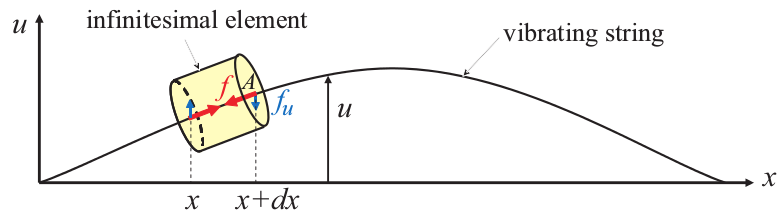
\includegraphics[scale=0.5]{fil-infinitesimal}
\caption{Application de la seconde loi de mouvement de Newton à un élémen infinitésimal d'un fil sous l'équation en dimension 1 $u_{tt} = c^2 u_{xx}$}
\label{figure/fil-infinitesimal}
\end{figure}

Par substitution, on peut vérifier facilement que $u(x,t) = a\,.\, f(x+ct) \,+\, b\,.\,f(x-ct)$ est la solution de l'équation de la vague pour une fonction arbitraire $f()$. Cette solution générale montre que des solutions particulières de l'équation de la vague sont les vagues voyageant avec une vitesse $c$ dans les mêmes directions. Le scalaire $c$, alors, représente la vitesse du son or la vitesse de la vague dans le matériel en question. Intuitivement, l'équation de la vague nous indique que ce matériel dans les régions à courbure positive est accéléré vers le haut alors que le matériel se trouvant dans les régions à courbure négative est accéléré par le bas. L'équation de la vague se généralise naturellement pour les dimensions supérieures. Pour des fluides "heightfields", nous nous intéressons particulièrement au cas de la dimension 2:

\begin{equation}
u_{tt} = c^2 (u_{xx} + u_{yy})
\end{equation}

qui est la forme spécifique en dimension 2 de l'équation plus générale $u_{tt} = c^2 \Delta u$ ou $u_{tt} = c^2 \nabla^2 u$. C'est une equation aux dérivées partielles de second ordre (DPE) qui nous montre comment le heightfield $u(x,y,t)$ à deux-plus-une dimensions évolue pendant le temps. Pour le résoudre, nous le remplaçons tout d'abord par deux EDP du premier ordre dans le temps:

\begin{eqnarray}
u_t & = & v\\
v_t & = & c^2(u_xx+u_yy)
\end{eqnarray}

Ensuite, nous discrétisons ce système d'équation en utilisant une grille régulière d'espacement $h$ et un pas de temps constant $\Delta h$, produisant:

\begin{eqnarray}
v^{t+1}[i,j] &=& v^{t}[i,j] + \Delta t\,\,c^2 (u[i+1,j] + u[i-1,j] + u[i,j-1] - 4\,\,u[i,j])\,\,/\,\,h^2\\
u^{t+1}[i,j] &=& u^t[i,j] + \Delta t \,\,v^{t+1}[i,j]
\end{eqnarray}

Nous avons rendu le schéma d'intégration plus stable qu'une étape de la méthode d'Euler explicite en échangeant l'ordre des instructions de mise à jour et en utilisant la nouvelle vélocité $v^{t+1}[i,j]$ pour les calculs des nouvelles positions, qui est des fois appelée une étape d'Euler semi-implicite.\newline

Maintenant nous sommes presque là où nous avions commencé avec certaines différences importantes de la version \textit{hello world} des fluides "heightfields". Cette version ne refroidit pas la vélocité. Le refroidissement est important et peut grandement faire augmenter la stabilité de la simulation. D'un autre côté, le refroidissement supprime les détails de hautes fréquences d'une animation. Nous avons aussi les paramètres significatifs $h$, $\Delta t$ et $c$ pour controller la simulation. Puisque nous avions utilisé l'intégration implicit d'Euler pour la discrétisation du temps, notre algorithme est seulement stable suivant \textit{certaines conditions}. En particulier, la condition de stabilité de \textit{Courant-Friedrichs-Lewy} maintient le fait que l'information doit traverser plus d'une cellule de la grille par pas de temps, i.e. $\Delta t < h$.\newline

De même, les conditions aux bords dans l'espace doivent être définies. Nous avons déjà eu affaire à une condition possible, appelée la condition du mirroir ou  la condition de la réflection. Jusque-là, nous avons répliqué les valeurs "height" au delà des bords   pour que les bords se comportent comme des murs qui reflètent les vagues. D'autres possibilités sont ceux qu'on appelle les \textit{conditions de bord périodiques}. Ici, nous imaginons que le domaine entier de la simulation à reproduire dans l'espace est formé de carreaux. Quand une valeur au delà du côté gauche du domaine est nécessaire, nous accédons à la cellule la plus à droite, i.e. réaliser une enveloppe autour. De cette façon, les vagues qui quittent le domaine de simulation d'un côté sont réintroduites d'un autre.\newline

Nous finissons ce chapitre sur les fluides "heightfield" avec des commentaires sur comment implémenter l'intéraction avec d'autres types d'objets et des bords plus généralisés.\newline

\begin{itemize}

	\item[$\bullet$] Le domaine de simulation n'est pas obligatoirement rectangulaire. Les conditions "mirroir" ou périodiques peuvent être appliquées à toute localisation d'une cellule marquée en tant que bord. Alors, en marquant une cellule arbitraire en tant que cellule de bordure, un domaine arbitraire peut être simulé.\\

	\item[$\bullet$] Un moyen d'implémenter l'interaction de fluides "heightfields" avec des systèmes de particules est d'absorber les particules qui sont en contact avec le haut d'une colonne d'eau. Dans ce cas, une certaine quantité d'eau est ajoutée à la colonne et la particule est supprimée. \cite{Obrien-95}\\
	
	\item[$\bullet$]L'intéraction des "heightfields" avec des corps rigides peut être simulée en laissant les corps rigides presser vers le bas les colonnes d'eau. Les colonnes d'eau en dessous des corps rigides ont besoin de pousser ces corps vers le haut. Elles peuvent faire cela en exerçant une force proportionnelle  à leurs surfaces représentées multipliée par la pression de l'eau en dessous de ce corps. La pression peut être calculée à partir de la différence en hauteur "height" de la colonne et la hauteur moyenne des colonnes.	
	
\end{itemize}

\chapter{Smoothed Particle Hydrodynamics}\label{chap:sph}

\section{Les systèmes de particules simples}

Comme discuté précédemment, pour les éclaboussures, les jets d'eau et les pulvérisations, la représentation en particules est le meilleur choix. Dans ces cas simples, il est souvent même nécessaire de simuler l'interaction des particules entre elles-mêmes. Nous appelons un système de particule sans interaction entre particules un système à particule \textit{simple}. Un tel système peut être implémenter très efficacement, c'est-à-dire qu'un grand nombre de particules peuvent être simulées en temps réel. Ce dont nous avons besoin est un ensemble de $N$ particules ($0 \leq i < N$) de masses $m_i$, de positions $x_i$, de vélocités $v_i$ et des forces extérieures accumulées $f_i$. Ces particules sont soit créées et initialisées avec des positions et des vélocités significatives avant que la simulation ne commence, ou générées pendant la simulation par des \textit{émetteurs}. Un émetteur génère typiquement les particules avec un certain débit [particule/s] et une certaine distribution de vélocité autour d'une direction principale. Pour s'assurer que les particules ne sont pas uniquement générées mais disparaissent au bout d'un certain  temps, elles ont une durée de vie définie. Quand la fin de leur durée de vie est proche, elles disparaissent discrètement. Leur durée de vie peut être également utilisée pour les teindre de couleur plus appropriée. Puisqu'il n'y a aucune interaction particule-particule, seules les forces propres des particules existent et l'équation dirigeante est formée d'équations différentielles ordinaires découplées:

\begin{eqnarray}
\dot{x_i} &=& v_i\\
\dot{v_i} &=& \frac{f_i}{m_i}
\end{eqnarray}

qui peuvent être efficacement intégrées en utilisant le schéma d'intégration implicite d'Euler par exemple.

\section{Intéractions particule-particule}

Si nous cherchons à simuler de petits amas d'eau avec des particules, il est bien essentiel que ces particules intéragissent entre elles. Sinon, elles s'amasseront à un point unique dans un coin ou suivant un pont. En général, une force d'interaction pour les particules prend la forme:

\begin{equation}
f(x_i, x_j) = F(|x_i - x_j|) . \frac{x_i - x_j}{|x_i - x_j|}
\end{equation}

où $F()$ est l'intensité de la force qui dépend uniquement de la distance entre les particules, sinon cela introduit un "torque". Un choix populaire est la force de \textit{Lennard-Jones} souvent employée dans les simulations dynamiques moléculaires:

\begin{equation}
f(x_i, x_j) = \left(\frac{k_1}{|x_i - x_j|^m} - \frac{k_2}{|x_i - x_j|^n} \right)  . \frac{x_i - x_j}{|x_i - x_j|}
\end{equation}

avec $k_1$, $k_2$, $m$ et $n$ sont des paramètres de contrôles. Les choix les plus usités sont $k_1 = k_2 = k$, $m = 4$ et $n = 2$.

Avec $N$ particules, il y a $O(N^2)$ interactions possibles dont on a besoin d'évaluer. Cette complexité quadratique peut être le grand blocage. Supposons que nous soyons capable de simuler dix milles particules sans interactions en temps réel. Cela signifie que nous aurions besoin de calculer maintenant cent millions d'interactions également en temps réel. Pour éviter cette complexité quadratique, nous introduisons une distance "cutoff"  $d$ au delà delaquelle les particules n'interagissent plus les unes par rapport aux autres. Dans le but de garder la simulation stable, il est important que la fonction $F()$ ne soit pas simplement reléguer ("cutoff to") à zéro à partir de la distance $d$ mais que cette fonction soit aussi continue $C^0$ et $C^1$ sur $d$. Maintenant à chaque pas de temps, les particules remplissent une grille régulière avec des espacements de cellules $d$. Après cela, les partenaires d'interaction potentielles pour une particule donnée se trouvent parmi les mêmes cellules ou celles adjacentes à elles. Si les particules sont également distribuées et que le nombre de particules par cellule se limite à une constante, les interactions peuvent être évaluées en temps linéaire.

\section{SPH}

La prochaine question à se poser est: pouvons nous faire mieux que d'utiliser les forces d'interaction de Lennard-Jones? Est-il possible d'utiliser les équations de Navier-Stokes et de les résoudre sur les particules? L a réponse est oui (\cite{muller-charypar-2003}). Le premier problème que nous avons à résoudre est de générer un champs continu et fluide à partir des grandeurs qui sont données uniquement pour les particules, i.e. dans des locations discrètes de l'espace. La méthode SPH (Smoothed Particule Hydrodynamics), originellement élaborée pour la simulation des étoiles \cite{monaghan-1992} résout ce problème. En son c\oe ur, il définit un moyen de lisser discrètement des champs d'attribut d'échantillon. Cela est effectué par ce qu'on appelle noyaux lissant "smoothing kernels" $W(r)$. La fonction noyau a besoin également d'être normalisée, c'est-à-dire que $ \int{W(| x-x_i|)dx} = 1 $.
Un choix populaire est le noyau \textit{poly6}:

\begin{equation}
W_{poly6}(r) = \frac{315}{64 \pi d^9} \left\{
\begin{array}{rl}
&(d^2 - r^2)^3 \;\; \mbox{ si } 0 \leq r \leq  d\\
&0 \:\:\:\:\:\:\:\: \mbox{ sinon } 
\end{array}
\right.
\end{equation}

parce que $r$ apparait uniquement au carré et qu'aucune racine carrée n'est à évaluer. Nous avons alors tous les ingrédients pour calculer un champ de densité lisse à partir des positions et des masses individuelles des particules:

\begin{equation}\label{equation/yields-density}
\rho (x) = \sum_{\scriptstyle j} m_j W(|x - x_j|).
\end{equation}

La masse volumique de la particule $i$ est simplement $\rho_i = \rho (x_i)$. Maintenant, il est plus évident de remarquer la nécessité de normaliser le noyaux. Avec cette restriction, la masse totale du système calculée comme l'intégrale du champ de masse volumique devient

\begin{equation}
\int \rho (x)dx = \sum_j \left( 
m_j \,\, \int W(|x - x_j|dx )
\right) = \sum_j m_j
\end{equation}

Après le calcul des valeurs des masses volumiques des particules individuelles, nous pouvons maintenant évaluer les champs lisses $A_s$ des attributs arbitraires $A_i$ des particules tels que:

\begin{equation}
A_s(x) = \sum_j m_j\,\, \frac{A_j}{\rho_j}\,\, W(|x - x_j|).
\end{equation}

Une propriété appréciable de cette formulation est que le gradient d'un tel champ peut être facilement évalué en remplaçant le noyau par le gradient du noyau:

\begin{equation}\label{equation/sph-99}
\nabla A_s(x) = \sum_j m_j\,\, \frac{A_j}{\rho_j}\,\,\nabla W(|x - x_j|).
\end{equation}

Dans une formulation Eulerienne (basée sur les grilles), les fluides sont décrites par un champs de vélocités $v$, un champ de masses volumiques $\rho$ et un champ de pression $p$. L'évolution de ces grandeurs à tout instant est donnée par deux équations. La première équation assure la conservation de la masse

\begin{equation}
\frac{\partial \rho}{\partial t} + \nabla . (\rho v) = 0
\end{equation}

alors que l'équation de Navier-Stokes formule la conservation de mouvement

\begin{equation}
\rho \left( \frac{\partial v}{\partial t} + v . \nabla v  \right) = - \nabla p + \rho g + \mu\,\, \nabla^2 v
\end{equation}

où $g$ est une force externe sur le corps et $\mu$ la viscosité du fluide. L'utilisation de particules à la place d'une grille stationnaire simplifie ces deux équations substentiellement. Premièrement, étant donné que le nombre de particules est constant et que chaque particule a une masse constante, la conservation de la masse est préservée et la première équation  peut être complètement ignorée. Deuxièmement, l'expression  $\frac{\partial v}{\partial t} + v . \nabla v $ dans le terme de gauche de l'équation de Navier-Stokes peut être remplacée par une dérivée substantielle $\frac{Dv}{Dt}$. Puisque les particules se déplacent avec le fluide, la dérivée substantielle du champ de vélocités se réduit simplement à la dérivée par rapport au temps de la vélocité des particules, ce qui signifie que le terme de convection $v.\nabla v$ n'est pas nécessaire pour des systèmes de particules.


Il restent les trois forces (dont l'unité est le $N.m^{-3}$) du terme de droite de l'équation de Navier-Stokes qui représentent la pression ($-\nabla p$), les forces externes ($\rho g$) et la viscosité ($\mu \nabla^2 v$). La somme des forces $f = -\nabla p + \rho g + \mu \nabla^2 v$ détermine  la modification du mouvement "momentum" $\rho \frac{partial v}{\partial t}$ de la particule sur le terme de gauche de l'équation. Pour l'accélération de la particule $i$ nous avons alors:

\begin{equation}
a_i = \frac{\partial v_i}{\partial t} = \frac{f_i}{\rho_i}
\end{equation}

où $v_i$ est la vélocité de la particule $i$ et $f_i$ et $\rho_i$  sont la force et le champ de masse volumique respectivement calculées de la particule $i$ sur une localisation donnée . Nous allons voir comment les forces appliquées sont évaluées en utilisant la méthode SPH.

\subsection{La pression}

L'application de la règle SPH décrite dans l'équation \ref{equation/sph-99} sur le terme  de pression $-\nabla p$ donne

\begin{equation}\label{equation/pressure-force}
f_i^{pressure} = - \nabla p(x_i) = - \sum_j m_j \frac{p_j}{\rho_j} \nabla W(|x_i - x_j|)
\end{equation}

Malheureusement, cette force n'est pas symétrique comme on peut le voir dans l'interaction de deux particules seulement. Puisque le gradient du noyau est zéro à son centre, la particule $i$ utilise uniquement la pression de la particule $j$ pour calculer sa force de pression et vice versa. Etant donné que les pressions sur ces localisations des deux particules ne sont pas égales en général, les force de pression ne seront pas symétriques. D'autres méthodes de symétrisation de l'équation \ref{equation/pressure-force} ont été proposé. Voici une solution très simple qui est à la fois stable et rapide à calculer:

\begin{equation}
f_i^{pressure} = - \sum_j m_j \frac{p_i + p_j}{2\rho_j} \nabla W(|x_i - x_j|)
\end{equation}

Puisque les particules portent uniquement les trois grandeurs masse, position et vélocité, la pression aux localisations de la particule doivent être évaluées en premier. Cela se fait en deux étapes. L'équation \ref{equation/yields-density} donne la masse volume à la localisation de la particule. Ensuite, la pression peut être calculer à partir de l'équation d'état des gaz parfait:

\begin{equation}
p = k(\rho - \rho_0)
\end{equation}

où $k$ est la constante des gaz qui dépend de la température et $\rho_0$ est la pression de l'environnement. Puisque les forces de pression dépendent du gradient du champ de pression, la différence (compensation) "offset"
 n'a aucun effet mathématiquement sur les forces de pression. Cependant, la compensation influence le gradient du champ lissé par la méthode SPH et rend la simulation numériquement stable.
 
 Cependant, l'incompressibilité n'est pas strictement imposée comme dans le cas de la simulation eulérienne. Les forces de pression ne sont que générées après le fait, quand les variations de la masse volumique eurent été formées. C'est clairement une méthode pénalisante et produit des comportement de rebond du fluide. Pour éviter cet effet, soit on peut prédire les masses volumiques et calculer les forces de pression sur les prédictions ou soit estimer la divergence du champ de vélocité en utilisant la méthode SPH et en résolvant l'équation de Poisson sur les particules \cite{premoze-2003}
 
 
\subsection{La viscosité} 
 
 L'application de la règle SPH sur  le terme de viscosité $\mu \nabla^2 v$ produit également des forces asymétriques
 
 \begin{equation}
 f_i^{viscosité} = \mu \nabla^2 v(x_i) = \mu \sum_j m_j \frac{v_j}{\rho_j} \nabla^2 W(|x_i - x_j|)
 \end{equation}
 
 parce que le champ de vélocités varie d'une particule à une autre. Puisque la force de viscosité dépend uniquement des différences de vélocité et non pas des vélocités absolues, il y a une manière naturelle de rendre symétriques les forces de viscosité en utilisant les différences de vélocités:
 
 \begin{equation}\label{equation/viscosity_symetrization}
 f_i^{viscosité} = \mu \sum_j m_j \frac{v_j - v_i}{\rho_j} \nabla^2 W(|x_i - x_j|)
\end{equation}  
 
 Une interprétation possible de l'équation \ref{equation/viscosity_symetrization}
est de voir les voisins de la particule $i$  à partir du frame de référence de mouvement de $i$ lui-même. Ensuite la particule $i$  est accélérée dans la direction de la vitesse relative de son environnement.


\subsection{Les forces externes}

Les forces externes comme la gravité, les forces de collision et les forces causées par l'interaction d'un utilisateur sont appliquées directement sur les particules comme le cas de systèmes de particules simples sans l'usage de SPH.

\section{Le rendu}

Il y a plusieurs méthodes pour faire le rendu des fluides qui sont définis comme des particules. Une des méthodes les plus simples et les plus rapides est l'utilisation de sprites. Si un filtre de lissage est appliqué sur les buffer profond "depth buffer" avant que les sprites soient dessinés, la granularité des particules peut être dissimulée à un certain degré. Un autre moyen de faire un rendu de particules fluides est de dessiner des isosurface du champ de masse volumique et de le triangulariser par un algorithme de "marching cubes". 

\newpage
\begin{thebibliography}{2}



\bibitem{premoze-2003}
Simon PREMOZE, Tolga TASDIZEN, James BIGLER, Aaron LEFOHN, and Ross WHITAKER:
\textit{Particle–based
simulation of fluids}.
In Comp. Graph. Forum (Eurographics Proc.), volume 22, pages 401–410, 2003.

\bibitem{monaghan-1992}
J. J. MONAGHAN:
\textit{Smoothed particle hydrodynamics}.
Annu. Rev. Astron. Astrophys., 30:543–574, 1992.

\bibitem{muller-charypar-2003}
Matthias M$\ddot{U}$LLER, David CHARYPAR, and Markus GROSS:
\textit{Particle-based fluid simulation for interactive
applications}.
In Proc. ACM SIGGRAPH/Eurographics Symp. Comp. Anim., pages 154–159, 2003.

\bibitem{Obrien-95}
J. O’BRIEN and J. HODGINS:
\textit{Dynamic simulation of splashing fluids}.
In Computer Animation, pages
198–205, 1995.

\bibitem{Hong-05}
Jeong-Mo HONG and Chang-Hun KIM:
\textit{Discontinuous fluids}.
ACM Trans. Graph. (Proc. SIGGRAPH),24:915–920, 2005.

\bibitem{harlow-65}
F. HARLOW and J. WELCH:
\textit{Numerical Calculation of Time-Dependent Viscous Incompressible Flow of
Fluid with Free Surface}.
Phys. Fluids, 8:2182–2189, 1965.

\bibitem{stam-99}
Jos STAM:
\textit{Stable fluids}.
In Proc. SIGGRAPH, pages 121–128, 1999.

\bibitem{fedkiw-stam-jensen-01}
R. FEDKIW, J. STAM, and H. JENSEN:
\textit{Visual simulation of smoke}.
In Proc. SIGGRAPH, pages 15–22, 2001.

\bibitem{foster-fedkiw-01}
Nick FOSTER and Ronald FEDKIW:
\textit{Practical animation of liquids}.
In Proc. SIGGRAPH, pages 23–30, 2001.

\bibitem{Selle-2005}
Andrew SELLE, Nick RASMUSSEN, and Ronald FEDKIW:
\textit{A vortex particle method for smoke, water and explosions}.
ACM Trans. Graph. (Proc. SIGGRAPH), pages 910–914, 2005.

\bibitem{osher-fedkiw-2002}
S. OSHER and R. FEDKIW:
\textit{Level Set Methods and Dynamic Implicit Surfaces}.
Springer-Verlag, 2002. New York, NY.

\bibitem{tsai-2002}
Yen-Hsi Richard TSAI:
\textit{Rapid and accurate computation of the distance function using grids}.
J. Comput. Phys., 178(1):175–195, 2002.

\bibitem{Jones-Baerentzen-sramek-2006}
M. JONES, A. B\AE RENTZEN, and M. SRAMEK:
\textit{3D distance fields: A survey of techniques and applications}.
IEEE Trans. Vis. Comp. Graphics, 2006.

\bibitem{sethian-1996}
J. SETHIAN:
\textit{A fast marching level set method for monotonically advancing fronts}.
Proc. Natl. Acad. Sci., 93:1591–1595, 1996.

\bibitem{tsitsiklis-1995}
J. TSITSIKLIS:
\textit{Efficient algorithms for globally optimal trajectories}.
IEEE Trans. on Automatic Control, 40:1528–1538, 1995.

\bibitem{zhao-2005}
Hongkai Zhao:
\textit{A fast sweeping method for Eikonal equations}.
Math. Comp., 74:603–627, 2005.

\bibitem{fournier-1986}
A. Fournier and W. T. Reeves:
\textit{A simple model of ocean waves}. In Proc. SIGGRAPH, pages 75–84, 1986.

\bibitem{hinsinger-2002}
D. Hinsinger, F. Neyret, and M.P. Cani:
\textit{Interactive animation of ocean waves}. In Proc. ACM SIG-
GRAPH/Eurographics Symp. Comp. Anim., pages 161–166, 2002.

\bibitem{jeffrey-2003}
A. Jeffrey:
\textit{Applied Partial Differential Equations}. Academic Press, 2003.


\end{thebibliography}

\end{document}
